\documentclass[acmsmall]{acmart}
\usepackage{amsmath}
\usepackage{diagbox}
\usepackage{graphicx}
\usepackage{listings}
\usepackage{textcomp}
\usepackage{tikz}
\usepackage{xcolor}

\usepackage{etoolbox} % toggle
\usepackage[capitalize,noabbrev,sort]{cleveref} % cref
\usepackage{listings}
\usepackage[caption=false]{subfig}
\usepackage{wrapfig}
\usepackage{listings}
\usepackage{url}
\usepackage{algorithm}
\usepackage{textcomp}
\usepackage{xspace}
\usepackage{hyperref}
\usepackage{mathpartir}
\usepackage{natbib}
\usepackage{diagbox}
\usepackage[normalem]{ulem} % needed for sout

\usepackage{tikz}
\usetikzlibrary{tikzmark,shapes.misc,decorations.pathmorphing}
\usepackage{mathtools}

%\usepackage[dvipsnames]{xcolor}
%\usepackage{lstparams, lstcoq}

\usepackage[export]{adjustbox} % makebox
\usepackage{multirow}
\usepackage{hhline}
\usepackage{pifont} % ding
\usepackage[inline]{enumitem}
\setlist{leftmargin=5.5mm,topsep=2mm}
\setlist[enumerate]{label=\textbf{(\arabic*)}}

\sloppypar
% avoid mid-page vertical stretch around wrap floats; slack goes to page bottom
\raggedbottom

%%%%%%%%%%%%%%%%%%%%%%%%%%%%%%%%%%%%%%%%%%%%%%%%%%%%%%%%%%%%%%%%%%%%%%%%%%%%%%%%
% Comments
%%%%%%%%%%%%%%%%%%%%%%%%%%%%%%%%%%%%%%%%%%%%%%%%%%%%%%%%%%%%%%%%%%%%%%%%%%%%%%%%

\newtoggle{comments}
%\toggletrue{comments}
\togglefalse{comments}

\setlength{\marginparwidth}{47pt}
\setlength{\marginparsep}{3pt}
\newcommand{\mpfont}{\scriptsize\sffamily}
\newcommand{\MPworker}[2]{
  \unskip{\color{#1}\vrule\vrule}
  {\marginpar{\raggedright\color{#1}\mpfont #2}}
}
\newcommand{\todo}[1]{
  \iftoggle{comments} {\MPworker{blue}{To-do: #1}} {}
}

%\newcommand{\todo}[1]{
%    \iftoggle{comments} {{\color{teal}[TODO: #1]}} {}
%}
\newcommand{\cancut}[1]{
  %    \iftoggle{comments} {{\color{orange}#1}} {#1}
  %{{\color{orange}#1}}
  {}
}

\newcommand{\namecomment}[3]{
  \iftoggle{comments} {\textbf{\textcolor{#2}{[#1: #3]}}} {}
}

% ADD YOUR NAME FOLLOWING THIS FORMAT
% Default color set:
%  red, green, blue, cyan, magenta, yellow, black, gray, darkgray, lightgray,
%  brown, lime, olive, white, orange, pink, purple, teal, violet.
\newcommand{\jiyong}[1]{\namecomment{Ji-Yong}{cyan}{#1}}
\newcommand{\toyifei}[1]{\namecomment{ATTN, YIFEI:}{red}{#1}}
\newcommand{\yifei}[1]{\namecomment{Yifei}{teal}{#1}}

%%%%%%%%%%%%%%%%%%%%%%%%%%%%%%%%%%%%%%%%%%%%%%%%%%%%%%%%%%%%%%%%%%%%%%%%%%%%%%%%
% Place holders
%%%%%%%%%%%%%%%%%%%%%%%%%%%%%%%%%%%%%%%%%%%%%%%%%%%%%%%%%%%%%%%%%%%%%%%%%%%%%%%%

\newcommand{\needcite}[1]{\textbf{\textcolor{red}{[cite: #1]}}}
\newcommand{\needref}[1]{\textbf{\textcolor{red}{[ref: #1]}}}
\newcommand{\ignore}[1]{}

%%%%%%%%%%%%%%%%%%%%%%%%%%%%%%%%%%%%%%%%%%%%%%%%%%%%%%%%%%%%%%%%%%%%%%%%%%%%%%%%
% Custom names
%%%%%%%%%%%%%%%%%%%%%%%%%%%%%%%%%%%%%%%%%%%%%%%%%%%%%%%%%%%%%%%%%%%%%%%%%%%%%%%%
\newcommand{\sysname}{\textsc{SemantiX}\xspace}
\newcommand{\sysnamelong}{semantic compatibility checking framework
between applications and compositions of distributed systems}

\newcommand{\sysgraph}{AppGraph\xspace}
\newcommand{\sysgraphs}{AppGraphs\xspace}

\newcommand{\sysmod}{DM\xspace}
\newcommand{\sysmods}{DMs\xspace}
\newcommand{\sysmodlong}{distributed system module}
\newcommand{\sysmodlongs}{distributed system modules}

\newcommand{\eg}{\emph{e.g.}, }
\newcommand{\ie}{\emph{i.e.}, }

\definecolor{StringRed}{rgb}{.637,0.082,0.082}
\definecolor{CommentGreen}{rgb}{0.0,0.55,0.3}
\newcommand{\greenCheck}{\textcolor{CommentGreen}{\ding{51}}}%
\newcommand{\redX}{\textcolor{StringRed}{\ding{55}}}%
\newcommand{\yellowTriangle}{\textcolor{olive}{\ding{115}}}%
\newcommand{\purpleTriangle}{\textcolor{purple}{\ding{115}}}%

\newcommand{\wcmark}{{\color{black}\ding{52}}}
\newcommand{\cmark}{{\color{blue}\ding{52}}}
\newcommand{\xmark}{{\color{red}\ding{56}}}

%%%%%%%%%%%%%%%%%%%%%%%%%%%%%%%%%%%%%%%%%%%%%%%%%%%%%%%%%%%%%%%%%%%%%%%%%%%%%%%%
% Custom enumerate/itemize/dictionary formats
%%%%%%%%%%%%%%%%%%%%%%%%%%%%%%%%%%%%%%%%%%%%%%%%%%%%%%%%%%%%%%%%%%%%%%%%%%%%%%%%
\usepackage{enumitem}

\newcommand{\enumparen}[1]{
  \begin{enumerate}[noitemsep,topsep=0pt]
      {#1}
  \end{enumerate}
}
\newcommand{\itemparen}[1]{
  \begin{itemize}[noitemsep,topsep=0pt]
      {#1}
  \end{itemize}
}
\newcommand{\customenumparen}[3]{
  \begin{enumerate}[label={#1},noitemsep,topsep=0pt,left=5pt..25pt]
      \setcounter{enumi}{#2}
      {#3}
  \end{enumerate}
}

%%%%%%%%%%%%%%%%%%%%%%%%%%%%%%%%%%%%%%%%%%%%%%%%%%%%%%%%%%%%%%%%%%%%%%%%%%%%%%%%
% Other formats
%%%%%%%%%%%%%%%%%%%%%%%%%%%%%%%%%%%%%%%%%%%%%%%%%%%%%%%%%%%%%%%%%%%%%%%%%%%%%%%%
\newcommand{\ballnumber}[1]{
  \tikz[baseline=(myanchor.base)]
  \node[circle,fill=.,inner sep=1pt] (myanchor)
  {\color{-.}\bfseries\footnotesize #1};
}

\newcommand{\circled}[1]{
  \tikz[baseline=(char.base)]{
    \node[shape=circle,draw,inner sep=1pt] (char)
    {#1};
  }
}

\newcommand{\para}[1]{\paragraph{#1}}
\newcommand{\subpara}[1]{\subparagraph{#1}}

%\newtheorem{assumption}{Assumption}

%%%%%%%%%%%%%%%%%%%%%%%%%%%%%%%%%%%%%%%%%%%%%%%%%%%%%%%%%%%%%%%%%%%%%%%%%%%%%%%%
% Fine grain edits
%%%%%%%%%%%%%%%%%%%%%%%%%%%%%%%%%%%%%%%%%%%%%%%%%%%%%%%%%%%%%%%%%%%%%%%%%%%%%%%%

% I'd rather add package "changes" but it conflicts with other
% things, so this is good enough.
% Prefix "sug" means "suggested"
\definecolor{SuggestionGreen}{HTML}{35713A} % taken from Google Docs
\newcommand{\suginsert}[1]{\textbf{\textcolor{SuggestionGreen}{#1}}}
% see https://tex.stackexchange.com/a/130626
\newcommand\sugdelete{\bgroup\markoverwith{\textcolor{SuggestionGreen}{\rule[0.35ex]{2pt}{0.35ex}}}\ULon}
\newcommand{\sugreplace}[2]{\suginsert{#1} \sugdelete{#2}}

%%%%%%%%%%%%%%%%%%%%%%%%%%%%%%%%%%%%%%%%%%%%%%%%%%%%%%%%%%%%%%%%%%%%%%%%%%%%%%%%
% Custom section/paragraph formats
%%%%%%%%%%%%%%%%%%%%%%%%%%%%%%%%%%%%%%%%%%%%%%%%%%%%%%%%%%%%%%%%%%%%%%%%%%%%%%%%
% titlesec removed for camera-ready: acmart v2.19 forbids redefining
% sectioning commands; we rely on acmart's native run-in \paragraph style.

\newcommand*{\squigglyarrowhead}[0]{\ \raisebox{0.15em}{\tikz \draw [->,
      line join=round,
      line width=0.8pt,
      decorate, decoration={
        zigzag,
        segment length=6,
        amplitude=.9,
        post=lineto,
        post length=1pt
}] (0,0) -- (0.4,0);}\ }
\newcommand*{\squigglyarrowtail}[0]{\ \raisebox{0.15em}{\tikz \draw [-,
      line join=round,
      line width=0.8pt,
      decorate, decoration={
        zigzag,
        segment length=6,
        amplitude=.9,
        post=lineto,
        post length=1pt
}] (0,0) -- (0.4,0);}\ }

\newcommand{\ltrans}[1]{\mathopen{\squigglyarrowtail} \hspace{-3pt}
\fbox{$#1$} \hspace{-3pt} \mathclose{\squigglyarrowhead}}
\newcommand{\lstep}[3]{#1 \mathop{\ltrans{#2}} #3}
\newcommand{\lstepStar}[3]{#1 \mathop{\ltrans{#2} \hspace{-3pt}^*} #3}
\newcommand{\llabel}[1]{\fbox{$#1$}}

\DeclareMathOperator*{\eventually}{\Diamond}
\DeclareMathOperator*{\always}{\Box}


\setcopyright{cc}
\setcctype{by-nc-nd}
\acmDOI{10.1145/3832138}
\acmYear{2026}
\acmJournal{PACMSE}
\acmVolume{3}
\acmNumber{ISSTA}
\acmArticle{ISSTA047}
\acmMonth{10}
\acmSubmissionID{issta26main-p405-p}
\received{2026-01-29}
\received[accepted]{2026-04-16}

\AtBeginDocument{%
  \providecommand\BibTeX{{%
Bib\TeX}}}

\begin{document}

\title{SemantiX: A Compatibility Checker between Applications and Compositions of Distributed Systems}

\author{Yifei Sun}
\orcid{0000-0002-1591-7458}
\affiliation{%
  \institution{Northeastern University}
  \city{Boston}
  \country{USA}
}
\email{yifei.sun@inria.fr}

\author{Ji-Yong Shin}
\orcid{0000-0002-1595-4849}
\affiliation{%
  \institution{Northeastern University}
  \city{Boston}
  \country{USA}
}
\email{j.shin@northeastern.edu}


\begin{abstract}
  Modern distributed applications compose multiple services with
different consistency guarantees. Mismatches between application
requirements and chosen system semantics can introduce subtle bugs,
but verifying compatibility across complex applications is both
challenging and time-consuming. In particular, existing testing approaches
or rigorous formal verification lacks flexibility and cannot
promptly provide correctness guarantees on multi-semantic compositions.

We present \sysname{}, a framework for checking semantic
compatibility between applications and compositions of distributed
systems with heterogeneous consistency models. \sysname{} embeds
formally defined distributed system modules of
consistency semantics which include the first formal definition of
visibility constraints. \sysname{} introduces the \sysgraph{} approach for
systematically modeling complex applications. Applications modeled
using \sysgraphs{} can be checked for their compatibility against a
combination of distributed system modules that the user is considering. 
Alternatively, \sysname{}
can search for combinations of modules compatible with the application.
We present three case studies on a movie streaming service, an
e-commerce platform, and a cross-service causal distributed storage service.
We demonstrate that \sysname{} can capture complex service compositions
with minimal encoding effort and quickly check compositional compatibility with
underlying systems or find the compatible system configurations. \sysname{}
enables developers to efficiently verify distributed application designs
and explore alternative consistency configurations, supporting more
agile development.

\end{abstract}

% CCS Concepts: https://dl.acm.org/ccs/ccs.cfm
\begin{CCSXML}
<ccs2012>
<concept>
<concept_id>10011007.10011074.10011099.10011692</concept_id>
<concept_desc>Software and its engineering~Formal software verification</concept_desc>
<concept_significance>500</concept_significance>
</concept>
<concept>
<concept_id>10011007.10010940.10010971.10011120</concept_id>
<concept_desc>Software and its engineering~Distributed systems organizing principles</concept_desc>
<concept_significance>300</concept_significance>
</concept>
<concept>
<concept_id>10003752.10003790.10003794</concept_id>
<concept_desc>Theory of computation~Automated reasoning</concept_desc>
<concept_significance>300</concept_significance>
</concept>
</ccs2012>
\end{CCSXML}

\ccsdesc[500]{Software and its engineering~Formal software verification}
\ccsdesc[300]{Software and its engineering~Distributed systems organizing principles}
\ccsdesc[300]{Theory of computation~Automated reasoning}

\keywords{consistency semantics, SMT solving, visibility}

\maketitle

\section{Introduction}

Modern cloud environments provide hundreds of services on various platforms
that are readily available for developers to build a
large-scale distributed application. System architects and developers
following the microservice or service-oriented designs can freely
choose and compose the building blocks in a modular fashion and plug them
into the application.

However, different distributed storage systems provide different consistency
semantics, and the mismatch of the chosen system's semantics and the
application's expected semantics could introduce subtle and silent
semantic bugs \cite{silentbugs, silentbugs2}. For example, a user may connect a
key-value store providing
eventual consistency to an application that expects a
linearizable storage service. In this case, the application could
read outdated information causing erroneous outcomes but without
crash-like explicit errors.

Developers and system architects could carefully review the
application needs and choose a
matching system. However, when the application depends on multiple
distributed services, checking the overall compatibility between the
application logic and multiple system components can easily become unmanageable. Even
if one successfully finds the correct combination, for example, through
extensive testing, developers might change the application code or
plug in different systems due to management, considerations of cost and performance.
Consequently, sophisticated compatibility checks must be repeated.

% When you have fixed application logic, you may choose two
% compatible systems. Two systems may collectively satisfy the
% application requirement, and changing one may invalidate both.
% NOTE: addressed below

Formal verification offers an alternative approach to these challenges,
where the correctness of the code can mathematically guarantee the
compatibility between code and system \cite{lampson2021hints}.
However, depending on
the complexity of the code, which could include non-essential parts
for reasoning about compatibility, the mechanized formal proofs
can take extensive time and effort \cite{certikos-osdi16,
klein2009sel4, wormspace}.
Furthermore, depending on the technique used, mechanized formal
proofs can be several times larger, in Lines of Code (LoC), than the implementation.
Moreover, minor changes can easily invalidate the entire proof
\cite{klein2009sel4}.
Thus, formal verification
leads to a similar problem to the above-mentioned testing methods where
the compatibility check
lacks the agility to adapt to changes in underlying systems and
applications.

In this paper, we propose \sysname{}, a lightweight \sysnamelong{}. \sysname{}
helps developers quickly encode their application logic and
requirements and check the compatibility with underlying distributed
systems using an SMT-based approach.
%to encode and analyze
%the safety properties of different consistency semantics and
%their compositions.

\sysname{} includes axiomatic models of distributed consistency
semantics, including eventual consistency,
linearizability~\cite{viotti2016consistency}, four session
guarantees~\cite{terry1994session}, pipeline RAM (PRAM) consistency~\cite{pram},
and causal consistency~\cite{causaldef}, which are commonly used in both
industry and academia~\cite{pileus, cosmosdb, anna, bayou, yogurt,
pnuts, cloudflare-session, causalmemory, cops}.
Users of our tool can leverage predefined models as
building blocks to rapidly iterate the service compositions and compatibility
of these models with their applications. Additional models can be
added to further
strengthen \sysname{}'s expressiveness with provided interfaces.
User-authored custom models inheriting from our base class automatically work with our pre-built ones,
including assertions for individual satisfiability and compatibility between one or more models
with user-defined application logic.

Although axiomatic definitions of distributed consistency semantics
exist in prior literature \cite{finkbeiner2007smt,
  tekken2017monitoring, kuper2019toward, fan2023satisfiability,
ma2024noctua}, encoding the details into the SMT
clauses for compatibility checks is challenging as the definitions
omit key details. For example, the commonly used concept
of \textit{visibility} for defining weak distributed consistency
semantics is subtle, but to our knowledge, no literature provides
a concrete definition. \sysname{} fills in these missing gaps to realize
full-fledged formal models for the compatibility checking.

Each application functionality is systematically encoded as a
directed acyclic graph (DAG), and the entire application is modeled as
a directed multi-graph format which we call the \sysgraph{}.
Each node in the \sysgraph{} represents key functionality in the application
that requires certain properties from the lower-level nodes it depends on,
and provides certain properties to the upper-level nodes.
The edges are used to specify more specific requirements and conditions that each
functionality needs to enforce in accessing the downstream nodes.
The leaf nodes typically represent external distributed services
following one of the pre-built distributed consistency semantic models
in \sysname{}.
%
The \sysgraph{} model is expressive enough to model an application logic
from high-level and trace complex dependencies that go across multiple
application logic boundaries, and distributed systems which the application
relies on. 

Using the \sysgraph{}, \sysname{} can verify simple applications 
relying on one distributed service and scale to complex microservice-based
production environments that leverage multiple modules and distributed storage systems.
%
Once the user specifies the application logic, \sysname{} can quickly
check the compatibility with the plugged-in consistency models. This
could be verifying the user's selection, or alternatively, \sysname{}
can explore different combinations of existing models to
find compositions of distributed systems with compatible consistency semantics.
These approaches enable fast exploration and iteration of alternative
system designs, guiding the development to adhere to intended
consistency guarantees from the very beginning.

%%%%%% Examples %%%%%%    % NOTE: addressed here
%%%%%% Examples %%%%%%    {
%%%%%% Examples %%%%%%      \color{red}
%%%%%% Examples %%%%%%      Consider a Not So Simple Storage Service
% (NS4) that advertises
%%%%%% Examples %%%%%%      itself to provide linearizability
% guarantee to users' read/write to objects.
%%%%%% Examples %%%%%%      NS4's architecture is based on an API
% layer that provides
%%%%%% Examples %%%%%%      arbitration between users and the
%%%%%% Examples %%%%%%      underlying monolithic storage layer
%%%%%% Examples %%%%%%      with read-your-writes guarantee. In this
% case, \sysname{} can be used to
%%%%%% Examples %%%%%%      model the abstract semantical properties
% of NS4, and check whether the
%%%%%% Examples %%%%%%      modeled NS4 have advertised user-facing
% linearizable guarantee.
%%%%%% Examples %%%%%%      Three nodes (client, API, and storage)
% and two edges (client to
%%%%%% Examples %%%%%%      API, API to storage) are
%%%%%% Examples %%%%%%      added to the DAG, where the client node
% requires linearizability
%%%%%% Examples %%%%%%      from the API node,
%%%%%% Examples %%%%%%      API node exports linearizability to the
% client, and API node
%%%%%% Examples %%%%%%      requires read-your-writes from the storage node.
%%%%%% Examples %%%%%%      The storage node exports read-your-writes
% to the API node. With
%%%%%% Examples %%%%%%      this modeling, \sysname{}
%%%%%% Examples %%%%%%      will be able to find a satisfying
% assignment for the DAG where
%%%%%% Examples %%%%%%      user-facing guarantee is linearizability.
%%%%%% Examples %%%%%%      However, if we swap the API layer
% requirement from the storage
%%%%%% Examples %%%%%%      layer from read-your-writes to
%%%%%% Examples %%%%%%      to PRAM consistency, \sysname{} will be
% able to find that the leaf
%%%%%% Examples %%%%%%      level semantical requirement can no
% longer be satisfied.
%%%%%% Examples %%%%%%    }

%%%%%% %%%%%%    \jiyong{Some challenges in doing this?}
%%%%%% %%%%%%    \yifei{What aspect should we talk about? Preliminary
% encoding on
%%%%%% %%%%%%      semantics? Debugging? Unresolved encoding on
% models with "eventual"
%%%%%% %%%%%%    visibility (see eventual source code)?}

As case studies, we use \sysname{} to model two microservice-based
applications \cite{gan2019an}, a movie streaming service, an e-commerce
service, and a cross-service causal storage system built on top of
multiple weakly consistent distributed storage systems \cite{boltoncc}.
We evaluate and demonstrate \sysname{}'s ability to check compatibility
between user-defined application specific logic, with underlying
distributed systems and explore other compatible semantics.
Our framework is capable of checking a single compatibility combination in under 200 milliseconds and exploring
other compatible combinations in less than 5 minutes.

%%%%%% %%%%%%    \jiyong{Some insights we gained?}
%%%%%% %%%%%%    \yifei{
%%%%%% %%%%%%      This is a project with a lot of moving parts,
% modeling a system,
%%%%%% %%%%%%      like in real life, have multiple ways to achieve
% the same goal.
%%%%%% %%%%%%      The level of abstraction we've chosen made it not
% too hard to check
%%%%%% %%%%%%      real system's behavior but that part is not implemented.
%%%%%% %%%%%%      Personally I feel like some part of the project
% would be better
%%%%%% %%%%%%      written in a proper theorem prover (representation
% of ops, binary
%%%%%% %%%%%%      relations), and discharge part of semantic
% constraints to SMT solvers.
%%%%%% %%%%%%    }

This paper makes the following contributions:
\itemparen{
%\item We present \sysname{}, the first compatibility checking tool for
%  applications that are composed of multiple distributed services.
\item We present \sysname{}, the first semantic-compatibility-checking tool 
	between an application and the multiple distributed services that it relies on.
\item We provide the missing formal definitions including visibility to fully express
  and check distributed weak consistency semantics.
\item We present a systematic way of encoding complex applications
  using the \sysgraph{} structure and checking their compatibility
  collectively using the SMT-based approach.
\item We conduct case studies on three representative distributed
  applications to demonstrate the workings of \sysname{}.
}

%%%%    % FIXME: full rewrite
%%%%    {\color{red}
%%%%
%%%%      Modern distributed systems often relax strict consistency
%%%%      guarantees to achieve
%%%%      scalability, fault tolerance, and low latency operations.
% Understanding and
%%%%      comparing different forms of relaxed consistency semantics
% is crucial for both
%%%%      system designers and researchers. Yet, systematically
% modeling and reasoning
%%%%      about these semantics, as well as their compositional
% properties, remained a
%%%%      understudied area.
%%%%
%%%%      Our framework aims to bridge this gap by providing a
% SMT-based approach to
%%%%      encode and analyze the safety properties of weaker consistency
%%%%      models (comparing
%%%%      with linearizability \cite{herlihy1990linearizability}), and their
%%%%      compositions under
%%%%      the assumption of livenss properties are always satisfied,
% i.e. eventual
%%%%      consistency \cite{petersen1997flexible} is guaranteed (replicas
%%%%      eventually converge),
%%%%      and we are layering everything on top of it. By offering a per-system
%%%%      (differentiated by symbols), logical representation of
% operations, our system
%%%%      can differentiates operations belonging to distinct systems
% and/or components
%%%%      through the use of unique symbols (see
% tests/test\_cross\_causal.py), enabling
%%%%      analysis of cross-system interactions. Additionally, solver
% backends can
%%%%      discharge proof witnesses on the satisfiability of specific
% consistency
%%%%      properties, or the compatibility and composability between
% multiple models.
%%%%      These approaches enable fast exploration and iteration of
% alternative system
%%%%      designs, guiding the development adhere to intended consistency
%%%%      guarantees from
%%%%      the very beginning.
%%%%
%%%%    }

\section{Background and Motivating Example}
\label{sec:background}

We first introduce the base distributed consistency semantics 
that \sysname{} models, and provide an example motivating our work.

\subsection{Background}

%\begin{wrapfigure}[12]{R}{3.3in}
\begin{wrapfigure}{R}{3.3in}
  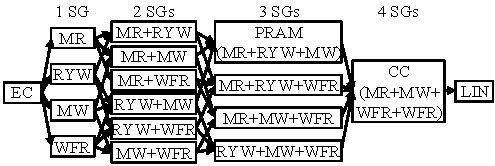
\includegraphics{figs/semantics-tree}
  \caption{Partially ordered semantics. Strictly stronger ones
    (destinations of the arrows) subsume the strictly weaker ones
  (sources of the arrows).}
  \label{fig:semantics-tree}
\end{wrapfigure}
Distributed consistency semantics define in which order updates are
applied and made visible in replica nodes within a cluster of
distributed system.
When an update request is submitted to the distributed system, a
subset (typically one) of nodes receives it and the update is
propagated across distributed nodes. Due to the asynchronous nature
of the network, replica nodes receive the update with
different delays and users accessing distinct nodes could observe
different data states. Distributed consistency semantics introduce
ordering constraints on top of such non-determinism so that
applications can predictably communicate with the system.

Among many distributed consistency semantics,
\sysname{} models seventeen widely used semantics in systems from both
industry and academia~\cite{pileus, cosmosdb, anna, bayou, yogurt,
pnuts, cloudflare-session, causalmemory, cops}, which includes eventual
consistency~\cite{burckhardt2014principles}, session
guarantees~\cite{terry1994session}, causal
consistency~\cite{causaldef}, and
linearizability~\cite{herlihy1990linearizability}.

While eventual consistency (EC) is considered a liveness property,
it defines a minimum safety property that visible data reflects valid
updates in history. Informally,
\itemparen{
\item \textbf{Eventual consistency (EC):} users may read any versions
  of data but with no incoming updates the most up-to-date version
  will eventually become visible to all reads.
}

Session guarantees (SGs), like its name, define semantics from the
viewpoint of a user session:
\itemparen{
\item \textbf{Monotonic reads (MR):} a user sees the same or later
  version of data than what was last seen by the same user.
\item \textbf{Read-your-writes (RYW):} a user sees the same or later
  version of data than what was last written by the same user.
\item \textbf{Monotonic writes (MW):} writes by a user apply in the
  order that this user wrote.
\item \textbf{Write-follows-reads (WFR):} writes by a user apply
  after writes corresponding to what this user read apply.
}
By choosing whether to enforce each of four session guarantees, a
total of 16 ($=2^4$) different semantics can be derived. While most
of them do not have specific names (e.g., MR + RYW), there are a few
well-known named semantics. For example, EC does not enforce any of
SGs, pipeline RAM consistency (PRAM) is a combination of MR, RYW, and
MW \cite{brzezinski2004session}, and causal consistency (CC) is a
combination of all four SGs, MR, RYW, MW, and
WFR \cite{sessiontocausal}. Still, PRAM \cite{pram} and
CC \cite{causaldef} have their own definitions:
\itemparen{
\item \textbf{PRAM consistency (PRAM):} read and write operations by
  a user happen in first in first out order from this user's point
  of view, but there are no global ordering guarantees.
\item \textbf{Causal consistency (CC):} read and write operations
  follow the causal ordering (or happens-before ordering~\cite{lamport1978time}) .
}
Finally, linearizability hides all distributed and concurrent natures
of distributed systems.
\itemparen{
\item \textbf{Linearizability (LIN):} all read and write operations
  are applied as if they are executed atomically by a single
  non-concurrent user.
}
These semantics can be partially ordered by their
strength~\cite{viotti2016consistency} where strictly stronger
semantics subsumes the weaker ones (\cref{fig:semantics-tree}). Thus,
when an application requires a certain semantics then a strictly
stronger one can safely replace the strictly weaker one without consistency violations.

\subsection{Motivating Example}
\label{subsec:eg}
Assume a movie streaming service built using a form of
microservice architecture where admins manage the serviced
content and clients rent movies and leave reviews~\cite{gan2019an}
(\cref{fig:case-study-media}).
There are quite a few functionalities and components to build the
service, and it is nontrivial to meet all service requirements
and to guarantee that all requirements are fulfilled.

For example, a movie metadata database (DB) stores list of
available movies and each movie's information such as the
logline, director, and cast. This DB is accessed 1) when
the service admin adds/modifies movie information and
2) when clients read the DB before renting a movie
or writing a movie review.

The developer of the system can choose an ACID database or linearizable
key-value store for the metadata DB, but this may not scale well as
stronger consistency models trade stronger data consistency guarantee with higher latency.
For utmost scalability and performance, an eventually consistent
key-value store can be used, but users may observe anomalies: for example, reviews
written to one replica may not be visible to the same user reading it.
Thus, to find a proper storage module, the key constraints are to identify
each access functionality, and to minimize anomalies users may experience.
For example, we can define admins must always observe their own
updates and clients must be able
to see what they have previously seen. These constraints
must be met by the consistency model of the metadata DB that the application developer chooses to use.
However, as functionalities of the system grow, constraints typically become
more sophisticated and the complexity of checking whether the constraints are fully satisfied by the 
DB also grows accordingly.

While the metadata DB example above is presented in isolation from
what a single DB service must satisfy, cross-DB constraints can exacerbate
the problem. For example, accessing the metadata DB would require
checking whether the user is an admin or a client with active movie subscription
status which may be maintained in a separate storage system. Thus,
dependencies from the login service and the user DB must be met:
the user must be able to observe the user's valid up-to-date status
and then access the other services. Renting a movie or reading/writing a
review involves additional consistency constraints that cross storage services
for movies and reviews forming more complex dependencies that the system as a
whole must satisfy.

\sysname{} provides facilities to systematically encode the constraints
and check whether the constraints are all satisfied.

\section{Distributed Consistency Models in \sysname{}}
\label{sec:design}

First, we present the theory and formal details regarding how we modeled
the distributed consistency semantics, and how applications can be
encoded into our \sysname{} framework, then further discharged to
SMT solvers like Z3 \cite{demoura2008z3} or CVC5 \cite{barbosa2022cvc5}.

%\subsection{Modeling Consistency Semantics}
\subsection{Preliminaries}

\sysname{} provides pre-built and pluggable \sysmodlongs{} (\sysmods{})
that represent distributed storage services, which can be checked individually or in group,
or as application constraints.
Each \sysmod{} models distributed consistency semantics introduced in
\cref{sec:background} and \cref{fig:semantics-tree}.
In the movie streaming service example, given all the constraints for the
metadata DB and the developer's \sysmod{} choice for the metadata DB,
\sysname{} can check if they are compatible. Also, given the constraints,
\sysname{} can search existing \sysmods{} for compatible
consistency semantics.

\sysname{} follows the definitions provided by
Viotti et al.~\cite{viotti2016consistency} and others
\cite{terry1994session, baldoni2002an, burckhardt2014principles}
and uses predicate logic derived from the definitions to
model \sysmods{} and reason about consistency semantics with SMT solvers.
Consistency semantics are defined as logical formulas over axioms and
relations. Each model enforces safety properties, specifically ordering and
visibility constraints on operations within history and abstract
executions.

\para{System Model and Assumptions.}
\sysname{} is a high-level semantic checker and is agnostic to concrete
implementations. It assumes an asynchronous network where messages may be
arbitrarily delayed, reordered, or dropped, and which may partition but not
permanently; nodes may crash but recover with their dependent state intact.
Operations are modeled as atomic request-response pairs in the sense that every
operation must have all of its fields populated. Non-atomic runtime behavior
such as cancellation or partial execution is expressed by setting the return
time to the interruption time and placing a partial or invalid marker in the
output value. Concurrency is captured by overlapping invocation-return intervals
(\cref{subsec:vis}). Object scope is per-semantic: relations that refer to
objects are quantified only within a single \sysmod{}'s constraints, and when
composing multiple \sysmods{} the cross-object correspondences are stated
explicitly as edge constraints (asserted as equality in our current
implementation). \sysname{} targets safety properties; liveness is out of scope.
A \sysname{} verdict is therefore only as trustworthy as these assumptions and
the faithfulness of the supplied \sysmods{} and \sysgraph{} to the real system.

\para{Operations, Relations, and History.}
To model a consistency semantics for a \sysmod{}, we must first define an
operation, a tuple containing the following:
\itemparen{
\item \textit{proc:} the process that issued the operation which is used for
  session identification.
\item \textit{type:} the type of the operation, such as read, write, or a
  \textit{custom} type. Custom types let user-defined \sysmods{} model operations
  that are neither a plain read nor a plain write (\eg read-modify-write or other
  application-specific actions) and constrain them with their own relations.
\item \textit{obj:} the object the operation is performed on.
\item \textit{ival:} operation's input value.
\item \textit{oval:} operation's output value or a special marker
  used for no output value.
\item \textit{stime:} invocation time of the operation.
\item \textit{rtime:} return time of the operation or a special
  marker used for non-returning operations.
}
An operation
can be conceptualized as an atomic action with a
request-response pair, where the request
is the operation itself and the response is the other operation with the
response time set.

Consistency semantics are typically defined using universally
quantified formulas
(e.g., $\forall a, b: \dots$) applied to relations that are treated
as uninterpreted
functions with constraints of operations by the SMT solver
(e.g., $\text{vis}(a, b)$, $\text{so}(a, b)$).
Typically, they are pairwise constraints defined over operations in a history $H$.
A history $H$ is a set of operations that have been logically executed in the
\sysmod{}.
The functions representing the relations are used as base premises
for consistency
models and are used in axioms and invariants that the SMT solvers
interpret and check. Given that we extensively use set comprehension to capture relations between operations, throughout the formalization, $a \xrightarrow{\text{rel}} b$ is denotationally equal to $(a, b) \in rel$, and directly translates to \texttt{rel(a, b)} in \sysname's source code.
Further, $rel^{-1}$ is equivalent to the inverse of $rel$ relation \cite{burckhardt2014principles,viotti2016consistency}.

The relations defined for operations within a history include:
\itemparen{
\item returns-before: $\text{rb} \triangleq \{(a, b) : a, b \in H
  \wedge a.\text{rtime} < b.\text{stime}\}$
\item same-session: $\text{ss} \triangleq \{(a, b) : a, b \in H \wedge
  a.\text{proc} = b.\text{proc}\}$
\item session-order:
  $\text{so} \triangleq \text{rb} \cap \text{ss}$
\item same-object: $\text{ob} \triangleq \{(a, b) : a, b \in H \wedge
  a.\text{obj} = b.\text{obj}\}$
}

In our implementation, each history relation function accepts an optional
\texttt{symbols} argument. This parameter allows users to
explicitly specify the symbolic operations, for example, \texttt{["a\_X",
"b\_X"]}, over which the relation's constraints should be quantified
for that specific instance \texttt{X}. This mechanism enables the application of
history-based constraints distinctly to operations belonging to
different modeled systems or components, contributing to the logical
isolation necessary for cross-system analysis.

\para{Abstract Execution (AE)}
An abstract execution instantiates and refines the history by
specifying which operations are visible to, or are arbitrated over
each other to model and check valid behaviors under a consistency semantics.
Abstract execution relations are non-deterministic
orderings used to capture more complex temporal constraints and
conflict resolution. The relationships include:
\itemparen{
\item \textit{Visibility (vis):} defines the effects of write propagation
  where the effect of
  an operation is visible to the process invoking another operation.
\item \textit{Arbitration (ar):} an application-specific, transitive and acyclic
  relation that provides a total order on conflicting operations,
  ensuring that observed executions follow a single coherent timeline.
\item \textit{Happens-before (hb):} used to capture probable causality,
  and is previously defined in the literature as the transitive union
  of session order and visibility: $hb \triangleq (\text{so} \cup
  {\text{vis}})^{+}$. We write $\text{acyclic}(hb)$ to require that $hb$ contains
  no cycle, i.e., no operation happens before itself, so that $hb$ is a strict
  partial order.
  \
}
The formal definitions of these relationships can be found in prior
work~\cite{burckhardt2014principles,viotti2016consistency}
with the exception of visibility which we define in \cref{subsec:vis}.
These relations provide the foundation
for modeling sophisticated consistency guarantees that go beyond
simple temporal ordering, enabling the specification of complex
distributed system behaviors where operations may be reordered,
delayed, or selectively visible across different system components.
In other words, multiple AEs are possible for a
single history as observed event orderings can differ between nodes.
The AE encode the non-determinism of asynchronous execution
environments and implementation-specific constraints.

\subsection{Base Consistency Semantics}
\label{subsec:semdef}

  %\begin{wrapfigure}[12]{R}{3.5in}
  \begin{wrapfigure}{R}{3.5in}
	 % \vspace{-0.2in}
  \begin{minipage}{3.5in}
    \begin{eqnarray*}
	    \text{MR} & \triangleq & \forall a \in H, \forall b, c \in H_\text{rd}: a
	    \xrightarrow{\text{vis}} b \land b \xrightarrow{\text{so}} c \Rightarrow
	    a \xrightarrow{\text{vis}} c
      \\
      \text{RYW} & \triangleq & \forall a \in H_\text{wr}, \forall b \in
      H_\text{rd}: a \xrightarrow{\text{so}} b \Rightarrow a
      \xrightarrow{\text{vis}} b
      \\
      \text{MW} & \triangleq & \forall a, b \in H_\text{wr}: a
      \xrightarrow{\text{so}} b \Rightarrow a \xrightarrow{\text{ar}} b
      \\
      \text{WFR} & \triangleq & \forall a, c \in H_\text{wr}, \forall b \in
      H_\text{rd}: a \xrightarrow{\text{vis}} b \land b
      \xrightarrow{\text{so}} c \Rightarrow a \xrightarrow{\text{ar}} c
      \\
      \text{PRAM} & \triangleq & \forall a, b \in H: a \xrightarrow{\text{so}}
      b \Rightarrow a \xrightarrow{\text{vis}} b
    \end{eqnarray*}
	  \end{minipage}
    \caption{Formal definitions of monotonic reads (MR), read-your-writes
      (RYW), monotonic writes (MW), write-follows-reads (WFR), and pipeline
    RAM (PRAM) consistency.}\label{fig:semdef}
  \end{wrapfigure}
Building on these preliminaries, we now discuss the formal definitions of
base consistency semantics: EC, MR, RYW, MW, WFR, PRAM, CC, and LIN. In
\cref{fig:semdef}, the semantics are defined axiomatically using the relations between
pairwise operations (i.e., $a, b, \textrm{ and } c$ in a history $H$ of
  operations, where $H_\text{rd}$ and $H_\text{wr}$ are histories of reads and
	  writes respectively).
  While we adopt the definitions of MR, RYW, MW, WFR,
  and PRAM of Viotti et al.~\cite{viotti2016consistency} (\cref{fig:semdef}),
  we introduce or augment EC, CC, and LIN for SMT encoding and
  check their correctness with respect to other semantic definitions
  using \sysname{}
  (Section \ref{sec:eval}).

  \para{Eventual Consistency (EC)}
  While EC definitions in other literature~\cite{terry1994session,
  eventual, viotti2016consistency}
  focus primarily on liveness aspects using the concept of
  eventual visibility of operations,
  \sysname{} concentrates on safety properties. Eventual visibility is a
  liveness property that requires reasoning over unbounded executions, which is
  considered hard, if not impossible, to express with finite SMT
  formulas; following the standard separation between
  safety and liveness~\cite{burckhardt2014principles}, \sysname{} therefore
  excludes it and models the two safety components of EC:
  (1) non-circular causality, an acyclic projection of the happens-before
  relation,
  and (2) contextual return value consistency, a predicate on abstract
  executions ensuring that the return value of any operation within
  that execution belongs to the set of its valid return values
  guided under the can-view relation which we define in \cref{subsec:vis}.
  \begin{align*}
    &\text{EC}(\mathcal{F}) \triangleq \text{acyclic}(hb) \land \forall
    op \in H: op.oval \in \mathcal{F}(op, ctx(A, op)) \\
    % for all read op, the ival of operations thats in can-view relation with op
    &\mathcal{F}_{\text{can-view}}(op, ctx(A, op)) = \{x.ival \in
    H_\text{wr} : (op, x) \in \text{can-view}\}
  \end{align*}
  Here, $ctx(A, op)$ denotes the context of $op$ in an abstract execution $A$
  (the operations visible to $op$), and the return-value function $\mathcal{F}$
  maps an operation and its context to the set of admissible return
  values~\cite{burckhardt2014principles, viotti2016consistency}. \sysname{}
  instantiates $\mathcal{F}$ with the can-view relation
  ($\mathcal{F}_{\text{can-view}}$), substituting possible visibility for the
  strict context $ctx(A, op)$ (an over-approximation), so that
  every operation's output is one of the input values of the writes it can view.

  \para{Causal Consistency (CC)}
  There is no single agreed-upon definition of causal consistency across the
  literature. Our CC formulation primarily follows the writes-into semantics of
  causal memory~\cite{baldoni2002an}, cross-checked against the definitions of
  Viotti et al.~\cite{viotti2016consistency} and Burckhardt et
  al.~\cite{burckhardt2014principles} rather than merging them. The
  \textit{writes-into (wi)}
  relation~\cite{baldoni2002an} connects write operations directly with the
  reads that retrieve their values. This guarantees that when
  a read operation observes a specific write, all following writes
  within the same session honor that causal sequence. The formalization
  coordinates session order, arbitration, visibility, and writes-into to
  preserve consistent causal histories.

  Operations belong to the \texttt{wi} set when: a write $a$
  writes into a read $b$ if and only if $b$ retrieves the value
  initially written
  by $a$, and $a$ and $b$ access the same object (or identical memory region).
  Each $b$ can have at most one corresponding $a$, maintaining acyclicity.
  When one operation succeeds another in session order, their
  relationship within the abstract execution faces additional constraints.
  Particularly, if $(a, b) \in \text{so}$, then $a$ must write-into $b$ when
  $b$ represents a read operation, and $a$ must be visible and
  arbitrated prior to $b$. Consequently, session order establishes a causal
  sequence that manifests in the relations wi, vis, and ar.
  %$$
  \begin{eqnarray*}
    \text{CC} \triangleq \text{WFR} \land \forall a, b \in H: (a, b) \in
    \text{so} \Rightarrow (a, b) \in \text{wi} \cap \text{vis} \cap \text{ar}
  \end{eqnarray*}
  %$$
  These constraints collectively establish a causal memory model where
  session order, observed values, and write sequences maintain
  alignment, ensuring
  causally dependent writes manifest in proper order from any
  observer's viewpoint.

  \para{Linearizability (LIN)} In our encoding of LIN,
  we introduce a modified single global order constraint to unify visibility and
  arbitration for all write operations regardless of operations in
  session-based semantics or not, and enforce real-time ordering to
  ensure that the observed histories comply with returns-before relations:
  i.e., linearization as operations come in instead of lazily ordering
  events when
  reads occur \cite{zhang2018building}.
  \begin{eqnarray*}
    \text{LIN} & \triangleq & (\forall a, b \in H: [a
      \xrightarrow{\text{vis}} b \implies a \xrightarrow{\text{ar}} b] \land  [a \xrightarrow{\text{ar}} b \land a.rtime < \infty \implies
    a \xrightarrow{\text{vis}} b]) \\
    & & \land \quad rb \subseteq ar \quad \land \quad \forall x \in H: x.oval \in \{y.ival \in H_\text{wr} : (x,
    y) \in \text{can-view}\}
  \end{eqnarray*}


  \subsection{Formal Definitions of Visibility}
  \label{subsec:vis}

%\begin{wrapfigure}[12]{R}{3.3in}
\begin{wrapfigure}{R}{3.3in}
%	\vspace{-0.1in}
\Small \centering
	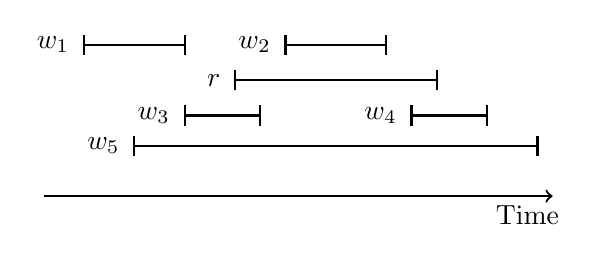
\begin{tikzpicture}[scale=0.64]
	  % time
	  \draw[->, thick] (0.2,1) -- (10.3,1);
	  \node[below] at (9.8,1) {Time};
	  \draw[thick] (1,4) -- (3,4);
	  \draw[thick] (1,3.8) -- (1,4.2); % left terminating bar
	  \draw[thick] (3,3.8) -- (3,4.2); % right terminating bar
	  \node[left] at (0.9,4) {$w_1$};
	  \draw[thick] (5,4) -- (7,4);
	  \draw[thick] (5,3.8) -- (5,4.2); % left terminating bar
	  \draw[thick] (7,3.8) -- (7,4.2); % right terminating bar
	  \node[left] at (4.9,4) {$w_2$};
	  % middle
	  \draw[thick] (4,3.3) -- (8,3.3);
	  \draw[thick] (4,3.1) -- (4,3.5);  % left terminating bar
	  \draw[thick] (8,3.1) -- (8,3.5);  % right terminating bar
	  \node[left] at (3.9,3.3) {$r$};
	  \draw[thick] (3,2.6) -- (4.5,2.6);
	  \draw[thick] (3,2.4) -- (3,2.8);   % left terminating bar
	  \draw[thick] (4.5,2.4) -- (4.5,2.8); % right terminating bar
	  \node[left] at (2.9,2.6) {$w_3$};
	  \draw[thick] (7.5,2.6) -- (9,2.6);
	  \draw[thick] (7.5,2.4) -- (7.5,2.8); % left terminating bar
	  \draw[thick] (9,2.4) -- (9,2.8);   % right terminating bar
	  \node[left] at (7.4,2.6) {$w_4$};
	  \draw[thick] (2,2) -- (10,2);
	  \draw[thick] (2,1.8) -- (2,2.2);   % left terminating bar
	  \draw[thick] (10,1.8) -- (10,2.2); % right terminating bar
	  \node[left] at (1.9,2) {$w_5$};
	\end{tikzpicture}
	%\vspace{-0.1in}
    \caption{The can-view relation captures the
      possible visibility between read and write operations. The
      read-write pairs $r$ and $w_{1-5}$ are defined based on their start and return times, 
      where the read can view the effect of the write operations.
	  %if they fall into one of the cases defined in the can-view relation.
	}
    \label{fig:can-view}
  \end{wrapfigure}
  One of our key contributions is formally defining visibility.
  Although visibility is used as part of defining almost all semantics in
  \cref{subsec:semdef} and \cref{fig:semdef}, its definitions in
  existing literature are informal and ambiguous regarding exact
  behavior under concurrent
  settings~\cite{viotti2016consistency,viotti2016towards,zhang2018building,ferreira2023antipode}.
  As with many seemingly simple informal definitions concerning
  concurrent and distributed environments, formally defining visibility
  for use in \sysname{}-like tools is non-trivial.
  We restructure visibility as a binary relation
  and perform case analysis on all possible combinations of
  read and write operations that can be \textit{visible} to each other.

  We introduce the notions of \textit{can-view} and \textit{viewed}
  to capture the
  deterministic and non-deterministic behavior of operations,
  and what it means for one operation to be able to \textit{observe}
  the effects of another operation. To achieve visibility, two
  operations must first fall in one of
  the categories in \textit{can-view}: either (1) the write 
  returns before the read (\eg $w_1$ and $r$ in \cref{fig:can-view}; 
  note that which process issued the read/write does not matter, as synchronization is not required to establish probable effect causality)
  or (2) the read and write are \textit{concurrent} (i.e., returns before relations do not hold as the durations of the read and write overlap 
  as in $r$ and $w_{2-5}$ in \cref{fig:can-view}) such that the read is eligible to observe the write's effect.
  %
  Formally, can-view is a binary relation over all pairs of operations. We
  constrain it only when a read $a$ and a write $b$ access the same object,
  based on their start and return times, and leave it unconstrained on every
  other pair:
  \begin{eqnarray*}
	  \text{can-view} \triangleq \{(a, b) : a \in H_\text{rd}, b \in H_\text{wr} \land a.\text{obj} = b.\text{obj}  \land 
		(b \xrightarrow{\text{rb}} a \lor \lnot(a \xrightarrow{\text{rb}} b \lor b \xrightarrow{\text{rb}} a))\}
  \end{eqnarray*}
%  \begin{equation*}
%	  (a, b) \in \text{can-view} \;\land\; a \in H_\text{rd} \;\land\; b \in H_\text{wr}
%	  \;\land\; a.\text{obj} = b.\text{obj} \;\Rightarrow\; (b \xrightarrow{\text{rb}} a
%	  \lor \lnot(a \xrightarrow{\text{rb}} b \lor b \xrightarrow{\text{rb}} a)).
%  \end{equation*}
  Using the invariant that every operation satisfies $\text{stime} \le
  \text{rtime}$, the case $b \xrightarrow{\text{rb}} a$ already implies
  $a.\text{rtime} \ge b.\text{stime}$, so this temporal condition reduces to the
  equivalent inequality $a.\text{rtime} \ge b.\text{stime}$: a read $a$ is
  eligible to view a write $b$ precisely when $a$ does not
  return before $b$ is invoked.
%%  \begin{eqnarray*}
%%	  \text{can-view} \triangleq \{(a, b) : a \in H_\text{rd}, b \in H_\text{wr} \land a.\text{obj} = b.\text{obj}  \land (b \xrightarrow{\text{rb}} a
%%	  \lor \textit{Concurrent}(a, b))\},
%%  \end{eqnarray*}

%%  where,
%%  \begin{align*}
%%	  \textit{Concurrent} & \triangleq & \{(a, b) : a, b \in H & \land \lnot(a \xrightarrow{\text{rb}} b \lor b \xrightarrow{\text{rb}} a)\}
%%  \end{align*}
%%  \begin{align*}
%%	  \textit{Concurrent} & \triangleq & \{(a, b) : a, b \in H & \land ((a.\text{stime} \geq b.\text{stime} \land a.\text{stime} \leq b.\text{rtime}) \\
%%	  & & & \lor  (a.\text{rtime} \geq b.\text{stime}  \land a.\text{rtime} \leq b.\text{rtime}) \\
%%	  & & & \lor  (a.\text{stime} \leq b.\text{stime} \land a.\text{rtime} \geq b.\text{rtime}))\}.
%%  \end{align*}
  %When two operations
  %$a$ and $b$ are defined to be in can-view relation
  %($a \xrightarrow{\text{can-view}} b$), either $a$ returned before
  % $b$, such that $b$'s write effect can be visible to $a$, or $a$ and
  % $b$ happened concurrently such that
  %$b$'s write effect might be visible to $a$.
 %% \begin{eqnarray*}
 %%   \text{can-view} & \triangleq & \{(a, b) : a \in H_\text{rd}, b \in H_\text{wr} \land a.\text{obj} = b.\text{obj} \\
 %%       & & \land ((a.\text{stime} > b.\text{rtime}) \\
 %%       & & \lor (a.\text{stime} \leq b.\text{stime} \land
 %%       	a.\text{stime} \leq b.\text{rtime} \land  a.\text{rtime} \geq b.\text{stime} \land
 %%       	a.\text{rtime} \geq b.\text{rtime}) \\
 %%       & & \lor (a.\text{stime} \geq b.\text{stime} \land a.\text{stime} \leq b.\text{rtime} \land 
 %%       	a.\text{rtime} \geq b.\text{stime} \land
 %%       	a.\text{rtime} \geq b.\text{rtime}) \\
 %%       & & \lor (a.\text{stime} \leq b.\text{stime} \land 
 %%         a.\text{stime} \leq b.\text{rtime} \land 
 %%         a.\text{rtime} \geq b.\text{stime} \land
 %%       a.\text{rtime} \leq b.\text{rtime}) \\
 %%       & & \lor (a.\text{stime} \geq b.\text{stime} \land
 %%         a.\text{stime} \leq b.\text{rtime} \land
 %%         a.\text{rtime} \geq b.\text{stime} \land
 %%         a.\text{rtime} \leq b.\text{rtime}
 %%       )
 %%   )\}
 %% \end{eqnarray*}

  While can-view captures the possible visibility between read and write, the
  resulting dependency between them is captured by the \textit{viewed} relation:
  \begin{eqnarray*}
    \text{viewed} & \triangleq & \{(a, b) : a \in H_\text{rd}, b \in
      H_\text{wr}  \land (a, b) \in \text{can-view} \quad \\
	  & & \land \text{ } ( (a.\text{oval} = b.\text{ival}) \quad \\
	  & & \text{ } \text{ } \lor (\exists x \in H_\text{wr} : 
	  	%(a, x) \in \text{can-view} \land 
		b.\text{obj} = x.\text{obj}  \land
		(b\xrightarrow{\text{rb}}x \lor \lnot(x \xrightarrow{\text{rb}} b \lor b \xrightarrow{\text{rb}} x)) \land a.\text{oval} = x.\text{ival})
      )
    \}
        %\text{ }(\exists x \in H_\text{wr} : (x, b) \in
        %\text{can-view} \land a.\text{oval} = x.\text{ival})
  \end{eqnarray*}
%%  \begin{eqnarray*}
%%    \text{viewed} & \triangleq & \{(a, b) : a \in H_\text{rd}, b \in
%%      H_\text{wr} \\
%%      & & \land (a, b) \in \text{can-view} \\
%%      & & \land (
%%        (a.\text{oval} = b.\text{ival})\lor \\
%%        & &
%%        \text{ }(\exists x \in H_\text{wr} : (x, b) \in
%%        \text{can-view} \land a.\text{oval} = x.\text{ival})
%%      )
%%    \}
%%  \end{eqnarray*}


  The viewed relation is defined as a non-deterministic
  pairwise partial ordering
  between a read and a write that builds upon can-view. Aside from timestamps
  falling into one of the can-view cases, we
  assign additional value-related constraints to operations: either the value
  written by the write operation must match the output
  of the read, or, in case of another write operation that happened after or
  concurrently to the aforementioned write (i.e., similar to can-view but between
  write pairs), the viewed relation enforces the
  output of the read to be from one of the writes (but only one can be chosen).
  In the visibility definition, the transitivity of the viewed relation
  is implicitly
  enforced.

  Using Figure \ref{fig:can-view}'s operations $r$ and $w_1$ as an example,
  since $r$ and $w_1$ are in the can-view relation, if $w_1$'s written
  value matches $r$'s output, then $r$ is in the viewed relation with $w_1$.
  Consider another operation $w_5$ in the same figure that happened
  concurrently with $w_1$. If $w_5$'s written value differs
  from $w_1$, but $r$'s output matches $w_5$'s input ($r.\text{oval} =
  w_5.\text{ival}$), then $r$ and $w_1$ are still in the viewed relation through
  the existential clause instantiated with $x = w_5$ (write $w_1$ still affects
  $r$). 
  %Here the write-write reference $(w_5, w_1) \in \text{can-view}$ is
  %unconstrained, so the operative condition is the existence of $w_5$ and the
  %value equivalence between $r$ and $w_5$.

  % actual vis
  Finally, the \textit{visibility (vis)} definition establishes a
  deterministic pairwise
  relationship between any two operations in the history
  rather than being limited to read-write pairs.
  It also adds the transitivity (propagation) and acyclicity
  (cannot go back in time) to the viewed relation.
  These were not enforced in our original viewed definition to preserve
  non-determinism in ordering concurrent operations and to include all pairs of
  operations that can be viewed by each other.
  When constraint $a \xrightarrow{\text{vis}} b$ is assigned to a pair
  of operations,
  the following four cases are considered:
  \begin{align*}
	  \text{vis} \triangleq & \{(a, b) : (a \in H_\text{rd}, b \in H_\text{rd} : \exists x \in
      H_\text{wr}: (x, a) \in \text{vis} \Rightarrow (x, b) \in \text{vis}) \\
      & \lor
      (a \in H_\text{rd}, b \in H_\text{wr} : \exists x \in
      H_\text{wr}: (x, a) \in \text{vis} \Rightarrow (x, b) \in \text{vis}) \\
      & \lor
      (a \in H_\text{wr}, b \in H_\text{rd} : (b, a) \in \text{viewed}
      \Rightarrow (a, b) \in \text{ar})  \quad \lor \quad
    (a \in H_\text{wr}, b \in H_\text{wr} : (a, b) \in \text{ar})\}.
  \end{align*}
  %\end{eqnarray*}
  Note that the read-read and read-write cases are recursively
  defined,
  %
  %where $a$ and $b$ are in $\text{vis}_\text{rd-rd}$ or
  %$\text{vis}_\text{rd-wr}$, if and only if there exists a
  %write $x$ that is
  %visible to $a$, and $x$ is in $\text{vis}_\text{wr-rd}$ or
  %$\text{vis}_\text{wr-wr}$ with $b$.
  %
  and we call this the
  write propagation rule. Conceptually, the rule implies that, if a read $a$
  and another operation (either read or write) $b$ are in the
  visibility relation,
  the closest write operation $x$ that is visible to read $a$ must
  be propagated to $b$. Whether this visibility relation can be satisfied
  depends solely on the existence of read $a$'s previous and
  immediately adjacent write operation $x$, and whether
  that $x$ can satisfy the write-read or write-write pairwise
  constraints of visibility.

  The write-read case is straightforward:
  %we term this rule definitive
  %visibility. Definitive visibility is defined as follows:
  if a write $a$ is visible to a read $b$, then $b$
  must have viewed $a$ and an arbitration relation must exist between
  $a$ and $b$
  to ensure the non-deterministic viewed relation has a
  linearization point, i.e., to cut off one of the possible paths in
  the viewed relation.
  We next define visibility between write operations. We call this
  propagation path write arbitration: whether two writes are visible to each other depends on the
  existence of an arbitration relation between them.
  Writes not ordered by visibility are considered invisible to each
  other~\cite{viotti2016consistency}
  and our proposed write arbitration resolves conflicts in concurrent and invisible operations.

  \para{Well-Formedness of Visibility.} Although visibility is defined
  recursively, the definition is well-founded. The read-read and read-write cases
  reference visibility only at a write-first position, which dispatches to the
  non-recursive write-read and write-write base cases in a single step, so the
  recursion depth is bounded by one. Acyclicity and transitivity are imposed as
  separate axioms on the resulting relation to enforce a strict partial order. In
  the SMT encoding, $\text{vis}$ is an uninterpreted function constrained by these
  axioms, and the solver searches for interpretations that satisfy them.

  With the complete visibility definition we encode the aforementioned semantics
  into \sysname{} which are then used to reason about the compatibility
  between applications and semantics/systems.

  %Operations do not contain the node that issued or
  %handled the operation; they are defined as generic entities that can
  %be issued by any node and handled by any node. To add constraints on
  %the nodes that can issue or handle an operation, the \sysname{} user
  %must define nodes and edges.

  %By assigning unique symbols to operations (and potentially
  % relations) associated
  %with different components (e.g., $a_X$, $b_X$, $\text{vis}_X$ for
  %System X; $a_Y$, $b_Y$, $\text{vis}_Y$ for System Y), we maintain
  %the necessary logical isolation. This ensures that the axioms and
  %constraints of a specific consistency model only apply to the
  %operations within that specific system's scope. This symbolic
  %separation is fundamental for enabling the analysis of
  %cross-system interactions, where specific ``glue''
  %constraints can then be added explicitly to relate operations across
  %these distinct symbolic domains, as demonstrated in our cross-causal
  %consistency modeling.

\section{\sysname{} Design}
\label{sec:usage}

We design the \sysmodlong{} (\sysmod{}) based on the definitions in
previous section. There are 2 main ways to interact with our framework,
(1) compatibility check and (2) compositional check. Compatibility check is specific
to \sysmods and is meant to assert the pairwise relationship between provided
arguments. Compositional checks are specific to applications involving
multiple components including \sysmods{} and are
built upon the compatibility check.
A \sysmod{} represents a single distributed system with specific semantics
and \sysname{} can perform individual \sysmod{} validation to check if all
semantic constraints are sound and compatible, as
well as pairwise checks between two \sysmods{} to determine if one
is satisfiable under another's constraints.
More importantly, \sysname{} can model applications that rely on multiple
distributed systems with different
consistency semantics (i.e., \sysmods{}) and can check for constraint satisfiability
between application logic and assigned semantics by performing a
compositional check using the \sysgraph{}.

\subsection{Compatibility Check}

\sysname{} is designed to reason about
compatibility among consistency semantics.
We define (pairwise) compatibility between two consistency semantics using \sysmods{}
$M_1$ and $M_2$ using
an implication-based criterion. $M_1$ is considered compatible with
$M_2$ if the formula $M_1 \Rightarrow M_2$ is valid, i.e., there is no
execution that satisfies all constraints of $M_1$ without also
satisfying $M_2$.
We implement this by asserting the negation $\neg (M_1 \Rightarrow M_2)$ and
checking if it is unsatisfiable using our SMT-based approach. If no
counterexample can be found, it implies that $M_1$
refines/subsumes $M_2$. This compatibility check is not symmetric:
$M_1 \Rightarrow M_2$
holding does not necessarily mean that $M_2 \Rightarrow M_1$ also holds.

Table \ref{tab:pairwise-time} shows a result of pairwise
compatibility checks for
base semantics in \sysname{} which in part shows that our consistency
models' compatibility faithfully matches with the theoretical results
in \cref{fig:semantics-tree} and in previous literature \cite{terry1994session}.

To combine multiple consistency models into a single stronger model, we used
logical conjunctions on each \sysmod{}'s constraints. By taking the constraints
representing each model's semantics and forming their conjunction, we derive a
aggregated model that enforces all included constraints simultaneously.
This approach allows incremental composition: users can start from a
base model and iteratively strengthen it by adding new sets of constraints,
either from our implemented models or user-defined constraints, representing
additional consistency guarantees.

\subsection{\sysgraph{} and Compositional Check}
%. Components (e.g., functionality)
%of an application are modeled as nodes and data flow and constraints
%between systems are represented as edges connecting the nodes in the
%\sysgraph{}. \sysname{} can check specific assignments of distributed
%system semantics or outputs results of all satisfiable assignments
%for the \sysgraph{}.

Applications that rely on multiple distributed systems with different
consistency semantics can be checked for correctness by performing a
compositional check using the \sysgraph{}.
Our compositional check
verifies if a distributed application, modeled as a graph (i.e,
\sysgraph{}) can have its components interact while 
respecting their individual consistency requirements and guarantees.

%The function checks if there exists at least one valid way to assign
%specific semantics (from the choices provided in needs/provs/cons)
%such that all interactions are consistent.

% The \sysgraph{} is composed of \textit{nodes} with two fields:
% (1) \textit{needs}, required constraint tuples from dependent components, and
% (2) \textit{provs}, constraint tuples it provides to other nodes.
% \sysname{} users can freely specify application logics, and each node
% has both \textit{needs} and \textit{provs}, with either our predefined built-in
% \sysmods{} or user-defined
% constraints that represent the node's semantics using our interface.
% \textit{Edges} connect nodes and have the \textit{cons} field,
% specific constraint tuples for the node pair interaction.
% In pluggable constraints for \textit{needs}, \textit{provs}, and \textit{cons},
% users may use (1) pre-build or bring-your-own \sysmods representing consistency semantics,
% (2) application-level and application-specific logic.
% The tuples within the list represent constraints that must hold together
% (logical \textsc{and}).

The \sysgraph{} (e.g., \cref{fig:case-study-media,fig:case-study-shop,fig:cross-service-causal}) 
consists of \textit{nodes} with two fields:
\textit{needs}, required constraint tuples from dependent components, and
\textit{provs}, constraint tuples provided to other nodes.
Each node's semantics can be expressed using (1) the predefined consistency \sysmods{}
and/or (2) user-defined/application-specific constraints that implement the same interface. Edges connect nodes
and carry \textit{cons}, constraint tuples for that node pair's interaction, where
each tuple is a conjunction of constraints. 

%For pluggable constraints in \textit{needs}, \textit{provs}, and \textit{cons},
%users can combine:
%(1) consistency semantics (pre-built or custom \sysmods{}), and
%(2) application-level or application-specific logic.

\usetikzlibrary{arrows.meta, positioning, calc, fit}

%\begin{wrapfigure}[22]{R}{3.3in}
\begin{wrapfigure}{R}{3.3in}
%\vspace{-0.2in}
\Small \centering
\centering
\begin{tikzpicture}[
  font=\footnotesize,
  node distance=8mm,
  u/.style={draw, rounded corners, fill=blue!10, align=center, inner sep=3pt},
  v/.style={draw, rounded corners, fill=green!10, align=center, inner sep=3pt},
  boxext/.style={draw, rectangle, align=left, inner sep=3pt},
  lbl/.style={font=\scriptsize},
  ->, >=Latex
]
\node[u] (u) {node $u$ \\ \textbf{needs} / provs};
\node[v, right=22mm of u] (v) {node $v$ \\ needs / \textbf{provs}\\{\scriptsize selects \textcolor{red!70!black}{\texttt{check\_provs}}}};
\node[draw, dotted, rectangle, fit=(u)(v), inner sep=6pt,
      label=above:{\scriptsize \sysgraph: needs/cons/provs}] (sel) {};
% path premise
\node[boxext] (path) [below=12mm of u, xshift=-3mm] {(accumulated) \\ \textcolor{orange!80!black}{$\texttt{path\_premise}$}};
% compat
\node[boxext, align=left, thick] (compat) [right=4mm of path] {%
\texttt{compatible(}\\
\quad \textcolor{red!70!black}{\texttt{check\_provs}},\\
\quad \texttt{compose(}\textcolor{blue!70!black}{\texttt{check\_needs}}\texttt{, }\textcolor{purple!70!black}{\texttt{check\_ec}}\texttt{)},\\
\quad \textcolor{orange!80!black}{\texttt{path\_premise}},\\
\texttt{)}};
% result
\node[boxext, align=center] (ok) [below=4mm of compat] {edge $(u,v)$ passes / discard};
% extract
\node[boxext, align=center] (extract) [left=12mm of ok] {\texttt{extract(...)}\\(optional aggregate)};
% inside app graph
\draw[->]
  (u) -- node[lbl, above] {select \textcolor{blue!70!black}{\texttt{check\_needs}}}
        node[lbl, below, align=center] {edge $(u,v)$\\select \textcolor{purple!70!black}{\texttt{check\_ec}}} (v);
% app graph to compatible args
\draw[->, dashed] (sel.south) -- (compat.north);
% path premise into compatible
\draw[->, dashed] (path.east) -- node[lbl, above] {} (compat.west);
% result
\draw[->, dashed] (compat) -- (ok);
\draw[->, dashed] (ok.west) -- node[lbl, above] {after} node[lbl, below] {success} (extract.east);

\end{tikzpicture}
%\vspace{-0.1in}
        \caption{Example flow for a single edge $(u,v)$: inside \sysgraph, select \texttt{check\_needs}, \texttt{check\_ec}, and the node’s \texttt{check\_provs}; outside, evaluate \texttt{compatible} on \texttt{compose(check\_needs, check\_ec)} and \texttt{path\_premise}. After a successful compatibility check, \texttt{extract} function can optionally aggregate \texttt{compatible} return value. For multigraphs, repeat per parallel edge (or edge combinations) with its own \texttt{cons} tuple. Solid arrows are part of \sysgraph and have the same meaning as the figures below. Dashed arrows represent control flow.}
\label{fig:skel}
\end{wrapfigure}


In the implementation (also see Fig. \ref{fig:skel}), we perform a depth-first search (DFS) starting from a
given source node, keeping track of visited edges and the accumulated
constraints in \texttt{path\_premise}, along the current path.
Constraints in \texttt{path\_premise} are invisible to users and are dynamic in nature based on which
edge(s), \texttt{needs}, \texttt{provs} are selected. Constraints are populated in and out
based on the satisfiability of the previous levels, and current level checks.
\sysname{} perform compatibility checks, \texttt{compatible(check\_provs,
compose(check\_needs, check\_ec), path\_premise)}:
for each edge $(u, v)$ from the current node $u$, it checks if \texttt{provs} from $v$
and \texttt{cons} from edge $(u, v)$ satisfy needs from $u$.
This checks if the chosen path satisfies the guarantees required by the destination
(\texttt{check\_provs}) is
implied by the conjunction (the result returned from call to \texttt{compose}) of the chosen needs of the
source (\texttt{check\_needs}) and the chosen edge constraints
(\texttt{check\_ec}),
considering the constraints already accumulated (\texttt{path\_premise}).
If all checks succeed, the application is deemed compatible
with the plugged-in \sysmods{} and the application logics are also
sound as a whole.


To avoid redundant checks in case of a subset of nodes and edges needs to be reused for scalability,
\sysname{} can aggretate a subgraph into a single logical node using the \texttt{extract} function.
% \jiyong{Does this previous sentence make sense?}
% \jiyong{What is composability check? Is it compatibility check or compositional check or something else?}
% same thing, prob missed it when revising the terms
After a successful compositional check, \texttt{extract} processes the resulting graph
representing a valid assignment of constraints, and outputs a single summary node.
This node encapsulates the net semantic guarantee of the subgraph reachable from the 
\texttt{entry} node, provided there are no external edges crossing the subgraph boundary.
The function performs a DFS starting from \texttt{entry} to compute this summary.
For each edge (\texttt{src}, \texttt{dst})
traversed in the DFS, the extraction function uses the specific \texttt{provs}
constraint assigned to \texttt{src} in the result graph, uses the specific
needs constraint assigned to \texttt{dst} in the provided graph, and retrieves
\texttt{cons} constraint assigned to the edge in
the argument graph. The extract function creates a composite constraint
for this single edge interaction: \texttt{compose(src\_provs, edge\_cons,
dst\_needs)}. This represents the conjunction of constraints relevant
to this specific step in the flow. It collects these composite
constraints from all edges reachable from subgraph root in the DFS. Finally,
it returns the logical \textsc{and} of all collected composite
constraints. Simply put, axioms and relations define constraints on
operations; similarly, \texttt{extract} defines a summary constraint on a
successfully composed subgraph. If the compositional check found a valid
way for components A, B, and C to interact starting from A,
\texttt{extract(A, graph)}---the first argument is aggregated subgraph's root node and the second is the return result from 
\texttt{compose} call, containing the full graph's nodes and edges---%
%(first argument is aggregate node's constraint flow entrance, second is the exit.
%Current implementation requires the first two arguments to be identical.
%The third is the return result from \texttt{compose} call, containing the full graph's nodes and edges)
% \jiyong{What does each arguement represent and how do they connect to components A B and C?}
generates a single formula representing the
overall guarantee provided by the A $\,\to\,$ B $\,\to\,$ C chain, as seen from A's
perspective, based on the specific choices made during the compositional check.
% Previously checked results are reusable with the above introduced extraction function
% \jiyong{If we do DFS do we ever get to reuse the checked results?}
%  not here because the "reuse" i mean is that, once the new aggregate node is created
% users can re-create a new full appgraph, so the intermediate steps of are skipped
% in new checks
By replacing a verified subgraph with its summary node, \sysname{} enables modular verification.
Subsequent checks on the full application graph can treat this summary as a primitive component,
thereby bypassing the internal complexity of the original subgraph and improving solver scalability.

\subsection{Compatible Combination Search}
\label{subsec:search}

\sysname{} is capable of searching for compatible \sysmods{} for an
application given an \sysgraph{}. When blank \sysmods{} are plugged into the
\sysgraph{}, \sysname{} searches for compatible combinations of
\sysmods{} for the user.
Considering that strictly weaker distributed semantics can be replaced
with strictly stronger ones and the weaker semantics are typically
more performant and cheaper to maintain, \sysname{} searches the space
in an order that prioritizes weaker semantics. Specifically, we give scores
0 to 5 to semantics in the columns from left to right in
\cref{fig:semantics-tree}
and test the combination that has lower sum of scores first during the search.
If compatible combinations are found, the search can stop early; replacing a
\sysmod{} in a compatible combination with a strictly stronger one is always
guaranteed to be compatible.
However, our search strategy is not optimal and investigating more
efficient search algorithms remains as future work.

%If a compatible combination is found that satisfies all unvisited edges
%between u and v at the current step, it adds the chosen constraints
%(needs, provs, cons) to the result graph, updates the path\_premise
%by composing the newly satisfied constraints, marks the edges as
%visited, and continues the DFS from the destination node v. If the
%DFS eventually visits all edges in the graph, the function returns
%True and the result graph showing one valid assignment. If a dead end
%is reached or no compatible combination works for an edge, it
%backtracks, removing the choices made at that step and trying other
%combinations. If the DFS completes without visiting all edges
%(meaning no fully consistent assignment was found), it returns False.

\section{Case Study}
\label{sec:cs}

To demonstrate \sysname{}'s utility, and to detail how a complex distributed
application can be specified in \sysname{} for the compatibility check with
pluggable distributed services, we present case studies of three applications.
Two applications, a movie streaming service and an online shopping
mall, are from
a microservice benchmark suite~\cite{gan2019an} and the other is from an
academic system that designs causally consistent storage service
across multiple weakly consistent distributed storage services~\cite{boltoncc}.
We mainly focus on the movie example to delve into the details.
Our framework is designed for a quick specification of applications
and prompt compatibility checks, and assumes users to be familiar with
axiomatic semantics and SMT encodings which are becoming more common and 
widely taught in schools~\cite{fmedu1, fmedu2, fmedu3, fmedu4}.

\subsection{Movie Streaming Service}


Our movie streaming service application~\cite{gan2019an} involves
multiple functionalities that can be represented as
regular nodes and edges in \sysgraph{} and distributed storage services (or DBs)
that can be captured as \sysmods{} (\cref{fig:case-study-media}).

\para{System Architecture.}
The media streaming service consists of eleven interconnected
components, each with specific consistency requirements based on
their functional roles. While users can choose a \sysmod{} for the
DB components, they must specify the constraints for the other components.

%\begin{wrapfigure}[25]{R}{2.8in}
\begin{figure*}
  \centering
	\begin{minipage}[c]{0.5\textwidth}
		\centering
  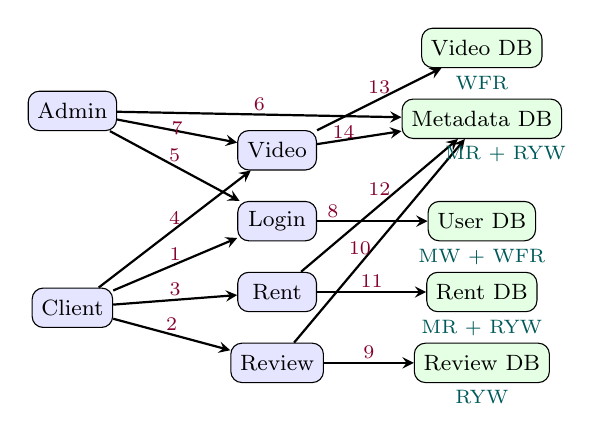
\begin{tikzpicture}[
      font=\footnotesize,
      node distance=1.8cm,
      service/.style={draw, rounded corners, fill=blue!10, minimum width=1cm, minimum height=0.5cm},
      storage/.style={draw, rounded corners, fill=green!10, minimum width=1cm, minimum height=0.5cm},
      arrow/.style={->, >=stealth, thick},
      label/.style={font=\small\itshape},
      app/.style={font=\scriptsize, text=purple!70!black},
      cons/.style={font=\scriptsize, text=teal!70!black}
    ]
    % client and admin
    \node[service] (client) at (0,0) {Client};
    \node[service, yshift=3mm] (admin) at (0,2.2) {Admin};

    % services
    \node[service] (login) at (2.6,1.1) {Login};
    \node[service] (review) at (2.6,-0.7) {Review};
    \node[service] (rent) at (2.6,0.2) {Rent};
    \node[service] (video) at (2.6,2.0) {Video};

    % db nodes
    \node[storage] (user_db) at (5.2,1.1) {User DB};
    \node[storage] (metadata_db) at (5.2,2.4) {Metadata DB};
    \node[storage] (review_db) at (5.2,-0.7) {Review DB};
    \node[storage] (rent_db) at (5.2,0.2) {Rent DB};
    \node[storage] (video_db) at (5.2,3.3) {Video DB};

    % edges from client
    \draw[arrow] (client) -- (login)       node[midway, above, app, yshift=-0.8mm] {1};
    \draw[arrow] (client) -- (review)      node[midway, above, app, yshift=-0.8mm] {2};
    \draw[arrow] (client) -- (rent)        node[midway, above, app, yshift=-0.8mm] {3};
    \draw[arrow] (client) -- (video)       node[midway, above, app, yshift=-0.8mm] {4};

    % edges from admin
    \draw[arrow] (admin) -- (login)        node[midway, above, app, yshift=-0.8mm] {5};
    \draw[arrow] (admin) -- (metadata_db)  node[midway, above, app, yshift=-0.8mm] {6};
    \draw[arrow] (admin) -- (video)        node[midway, above, app, yshift=-1.8mm] {7};

    % service to DB edges
    \draw[arrow] (login)   -- (user_db)     node[midway, above, app, yshift=-0.8mm, xshift=-0.5cm] {8};
    \draw[arrow] (review)  -- (review_db)   node[midway, above, app, yshift=-0.8mm] {9};
    \draw[arrow] (review)  -- (metadata_db) node[midway, above, app, yshift=-3mm, xshift=-2.5mm] {10};
    \draw[arrow] (rent)    -- (rent_db)     node[midway, above, app, yshift=-0.8mm] {11};
    \draw[arrow] (rent)    -- (metadata_db) node[midway, above, app, yshift=-0.1mm] {12};
    \draw[arrow] (video)   -- (video_db)    node[midway, above, app, yshift=-0.6mm] {13};
    \draw[arrow] (video)   -- (metadata_db) node[midway, above, app, yshift=-1.4mm, xshift=-2mm] {14};

    % consistency semantics
    \node[below=0.15cm, align=center, cons, yshift=-0.8mm] at (user_db) {MW + WFR};
    \node[below=0.15cm, align=center, cons, xshift=3mm, yshift=-0.8mm] at (metadata_db) {MR + RYW};
    \node[below=0.15cm, align=center, cons, yshift=-0.8mm] at (review_db) {RYW};
    \node[below=0.15cm, align=center, cons, yshift=-0.8mm] at (rent_db) {MR + RYW};
    \node[below=0.15cm, align=center, cons, yshift=-0.8mm] at (video_db) {WFR};
  \end{tikzpicture}
	\end{minipage}
	\begin{minipage}[c]{0.48\textwidth}
		\centering
  \caption{Architecture of the media streaming service with
    consistency guarantees. The numbers denote application
    constraints/flow, node labels on storage systems show
    provided consistency. Edges:
    1–4: Client requests to services (login, review, rent, video).
    5: Admin login.
    6: Admin updates metadata.
    7: Admin uploads video.
    8: Login service accesses User DB.
    9: Review service writes to Review DB.
    10: Review checks content existence in Metadata DB.
    11: Rent updates Rent DB.
    12: Rent checks content availability in Metadata DB.
    13: Video service accesses Video DB.
    14: Video service verifies metadata before playback.
}
  \label{fig:case-study-media}
	\end{minipage}
		%\vspace{-0.3in}
\end{figure*}
%\end{wrapfigure}



\begin{enumerate}[leftmargin=*,noitemsep,topsep=2pt]
  \item \textbf{Client and Admin}: These components represent the
    entry points for regular users and administrative personnel,
    respectively. They don't enforce specific consistency guarantees
    themselves but rely on the guarantees provided by the services
    they interact with.

  \item \textbf{Authentication}: Involves two nodes for clients and admins to authenticate.
    \begin{itemize}[leftmargin=*, noitemsep,topsep=0pt]
      \item \textbf{Login Service}: Manages user authentication and
        session handling. It requires order preserving writes
        for correct credential update and the user's updates
        (e.g., subscription status change) must always be visible for
        flawless service.
      \item \textbf{User DB}: Stores user credentials and
        profile information.
        %MW and WFR ensures
        %that when users update their profiles or credentials, these
        %changes are consistently visible to subsequent operations.
    \end{itemize}

  \item \textbf{Content Management}: Movie-related contents made accessible to clients by the admin.
    \begin{itemize}[leftmargin=*, noitemsep,topsep=0pt]
      \item \textbf{Video Service}: Handles video streaming requests
        and requires users to observe their own prior operations to ensure
        consistent content delivery.
      \item \textbf{Metadata DB}: Stores information about
        available videos (titles, descriptions, genres, etc.).
        %        with Monotonic Reads (MR) and Read Your Writes (RYW)
        %        guarantees. This allows administrative updates to be
        %        immediately visible while tolerating some staleness
        % for user reads.
      \item \textbf{Video DB}: Stores the actual video contents.
%        with WFR guarantees to maintain version consistency.
    \end{itemize}

  \item \textbf{User-Centered Functions}: Mostly hosts client-driven activities. 
    \begin{itemize}[leftmargin=*, noitemsep,topsep=0pt]
      \item \textbf{Review Service}: Manages user reviews; reviews should be immediately visible to the writer.
      \item \textbf{Review DB}: Stores user reviews.
        %with RYW
        %guarantees, allowing users to see their own reviews
        %immediately while other users might see slightly stale data.
      \item \textbf{Rent Service}: Handles media rental transactions;
        users must see their activities immediately.
      \item \textbf{Rent DB}: Records rental transactions.
        %with MR and RYW guarantees to maintain consistent transaction history.
    \end{itemize}
\end{enumerate}

\para{Constraint Encoding.}
We focus on the login and review services in \cref{fig:case-study-media}
to explain how constrains are encoded in \sysname{}.
In this example, the application requires that all users must register for
an account before they can log in, this would result in a request from
client to login service (edge 1), then to user database (edge 8).
If users want to post a review (edge 2), they must
be logged in (edge 1), and the review service must verify that the
title exists
in the metadata database (edge 10) before allowing the review to be
written (edge 9).
This represents a clear dependency chain in the media service example.
This dependency chain creates a cascading effect throughout the system
where each operation builds upon the successful completion of its
prerequisites.
The registration-before-login dependency establishes user identity,
the login-before-content-access dependency establishes authorization,
and the content-validation-before-review dependency establishes
referential integrity.


We next show the interaction flow from user login through posting a review
and formalize the corresponding edge constraints.
Semantically, 6 nodes are interacting with each other (client,
  login service, user database, review service, metadata database,
and review database) in the aforementioned dependency chain.
The edges between these nodes represent the flow of API requests and we
encode the prerequisites of each request as constraints on edges.
%Implementation-wise, 
Note that all constraints on edges can be
directly added to the nodes.
%encoded on the nodes 
%along with our
%predefined semantics. 
However, when modeling services with complex interactions 
with cross storage system dependencies, 
edge constraints can clearly
separate the providing/requiring constraints from downstream
%implementation-specific
service logic. In the implementation, we defined multiple operations
with read or write type to represent interactions between client,
service nodes, and storage nodes.
Formally, we can represent client's login operation (edge 8) as follows:
%\vspace{-0.1in}
% old version with linefeed
% \begin{align*}
%   EC_{login} &\triangleq \forall op_{login} \in H_{rd} : \exists
%   op_{reg} \in H_{wr} :\\
% &ob(op_{login}, op_{reg}) \land vis(op_{reg}, op_{login}))
% \end{align*}
% new version wo linefeed and consistent notation
\[
  EC_{\text{login}} \triangleq \forall op_{\text{login}} \in H_{\text{rd}} : \exists op_{\text{reg}} \in H_{\text{wr}} :
  (op_{\text{login}}, op_{\text{reg}}) \in ob \quad \land \quad (op_{\text{reg}}, op_{\text{login}}) \in vis.
\]
Since all interactions to User DB pass through Login, and Login node do not have cross
edges to outside graph components other than User DB, the subgraph Login, User DB and
edge 8 can be aggregated with \texttt{extract} function.

For services initiated from the client side, we modeled the behaviors
as a set of reuseable common constraints with the return-before
binary relationship. Formally:
% old version with linefeed
% \begin{align*}
% EC_{auth} &\triangleq rb(op_{login}, op_{rdreview}) \land
% rb(op_{login}, op_{wrreview}) \\
% &\land rb(op_{login}, op_{rent}) \land rb(op_{login}, op_{watch})
% \end{align*}
% new version with linefeed and consistent notation
% this is too wide
\begin{align*}
  EC_{\text{auth}} &\triangleq
  (op_{\text{login}}, op_{\text{rdreview}}) \in rb \quad \land \quad
  (op_{\text{login}}, op_{\text{wrreview}}) \in rb \\ 
	&\land \quad (op_{\text{login}}, op_{\text{rent}}) \in rb \quad \land \quad
  (op_{\text{login}}, op_{\text{watch}}) \in rb.
\end{align*}
The common constraints are then added to each edge that is dependent on the
login service or refer to the login operation, ensuring the chain
of dependencies is respected throughout the system.

For posting reviews,
the review service must first verify that the content exists in the
metadata database before allowing the review to be written. Similar to
the login operation, we can represent the review service's interaction
as a set of constraints with existential quantification, object constraints,
and return-before relationships, on top of consistency semantics
encoded at each nodes' provide and need fields. Formally,
\begin{align*}
EC_{\text{review}} &\triangleq \forall op_{\text{review}} \in H_{\text{wr}} : \exists op_{\text{rdmeta}} \in H_{\text{rd}} :\\
&(op_{\text{review}}, op_{\text{rdmeta}}) \in ob \quad \land \quad (op_{\text{rdmeta}}, op_{\text{review}}) \in rb.
\end{align*}

Following these practices one can specify relatively complex and construct \sysgraph with \sysmods and application-level constraints.
\sysgraph construction is straightforward, we instantiate nodes with their
\texttt{needs}/\texttt{provs} and connect them with edges carrying the above constraints.
Moreover, depending on system designers' requirements, Login node, User DB, and edge 8 can be collapsed into a single
aggregated node by applying \texttt{extract} (introduced in \cref{sec:background}) to the subgraph accumulates
both the semantic constraints (MW+WFR) and the application constraint $EC_{\text{login}}$ into one summary \texttt{provs}/\texttt{needs} tuple.
This lets us reuse the combined guarantee downstream or use it as a portable node in another \sysgraph.

%The example already specifies satisfiable \sysmods{}, but users can
%test other \sysmods{} or ask \sysname{} to search for the compatible
% \sysmods{}.

\para{Requirements and Compatibility Verification.}
Each component in the system requires consistency guarantees
from the DBs:% based on its functional role:
\begin{itemize}
\item The User DB provides MW and WFR guarantees, ensuring
  that credential updates are properly sequenced and visible, which
  is critical for authentication security.
\item The Metadata DB provides MR and RYW guarantees,
  balancing immediate visibility of administrative updates with
  tolerance for some staleness in user reads.
\item The Review DB provides RYW guarantees, prioritizing the
  user experience of seeing one's own reviews immediately while
  accepting eventual consistency for other users' views.
\item The Rent DB provides MR and RYW guarantees, ensuring
  consistent transaction records for both administrative and user views.
\item The Video DB provides WFR guarantees, maintaining
  version consistency for content delivery.
\end{itemize}

The edges in our model represent not just data flow but also critical
operational constraints. For example, the edge from the Client to the
Login Service carries the constraint that ``User must register before
login'', enforced through a visibility relationship between
registration and login operations. Similarly, the edge from the
Review Service to the Metadata Database enforces the constraint that
``Check metadata before reading reviews'', ensuring that reviews are only
accessible for valid content.

When we apply the compositional check to this system,
starting from the client node, it successfully verifies that the
composition of these services with their respective consistency
guarantees satisfies the overall system requirements.
This verification confirms that despite the heterogeneous consistency
guarantees across different components, the system as a whole
maintains its required properties.
For instance, the login flow
correctly enforces that registration must precede login, and the
review system correctly ensures that users can immediately see their
own reviews. %while maintaining content validity checks.

\subsection{Online Shopping Mall}
%
%
%\begin{wrapfigure}[10]{R}{2.8in}
\begin{figure}
  \centering
	\begin{minipage}[c]{0.56\textwidth}
		\centering
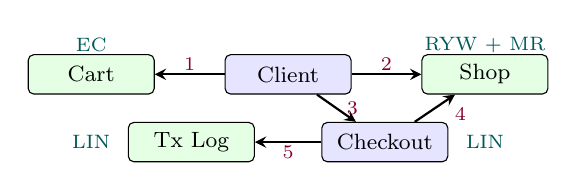
\begin{tikzpicture}[
    font=\footnotesize,
    node distance=1.2cm,
    service/.style={draw, rounded corners=2pt, fill=blue!10, minimum width=1.6cm, minimum height=0.5cm, align=center},
    storage/.style={draw, rounded corners=2pt, fill=green!10, minimum width=1.6cm, minimum height=0.5cm, align=center},
    arrow/.style={->, >=stealth, thick},
    app/.style={font=\scriptsize, text=purple!70!black},
    cons/.style={font=\scriptsize, text=teal!70!black}
  ]

  % nodes
  \node[service] (client) at (-0.3,0) {Client};
  \node[storage] (cart) at ([shift={(180:2.5cm)}]client) {Cart};
  \node[storage] (shop) at ([shift={(0:2.5cm)}]client) {Shop};
  %\node[service] (arbitrator) at ([shift={(315:1.77cm)}]client) {Checkout};
  %\node[storage] (tx) at ([shift={(225:1.77cm)}]client) {Tx Log};
  \node[service] (arbitrator) at ([shift={(325:1.5cm)}]client) {Checkout};
  \node[storage] (tx) at ([shift={(215:1.5cm)}]client) {Tx Log};

  % edges
  \draw[arrow] (client) -- (cart)       node[midway, above, app, yshift=-0.8mm] {1};
  \draw[arrow] (client) -- (shop)       node[midway, above, app, yshift=-0.8mm] {2};
  \draw[arrow] (client) -- (arbitrator) node[midway, right, app] {3};
  \draw[arrow] (arbitrator) -- (shop)   node[pos=0.35, right=0.2cm, yshift=-0.2mm, app] {4};
  \draw[arrow] (arbitrator) -- (tx)     node[midway, below, app, yshift=0.8mm] {5};

  % semantics
  \node[cons, align=center, yshift=1.2mm] at (cart.north) {EC};
  %\node[cons, align=left, right=1mm] at (shop.east) {RYW + MR};
  \node[cons, align=center, yshift=1.2mm] at (shop.north) {RYW + MR};
  \node[cons, align=left, right=1mm] at (arbitrator.east) {LIN};
  \node[cons, align=right, left=1mm] at (tx.west) {LIN};
\end{tikzpicture}
	\end{minipage}
	\begin{minipage}[c]{0.42\textwidth}
		\centering
\caption{Architecture of the online shopping system with consistency guarantees. Numbers denote application constraints/flow on edges: 1: client read/write cart; 2: client browse shop; 3: client purchase via checkout; 4: checkout check/update shop; 5: checkout record to Tx Log. Node labels show provided consistency semantics.}
\label{fig:case-study-shop}
	\end{minipage}
\end{figure}
%
%
An e-commerce application~\cite{gan2019an} is similar to the movie
streaming service but its architecture and constraints are simpler
(\cref{fig:case-study-shop}).
\para{Architecture.}
The online shopping application consists of five key components and only
models client behaviors:
\begin{enumerate}[leftmargin=*, noitemsep,topsep=0pt]
\item \textbf{Client}: The end-user interface through which
  customers browse products, manage their shopping cart, and
  initiate purchases. The client itself doesn't enforce specific
  consistency guarantees but relies on the interacting
  services' guarantees.
\item \textbf{Cart DB}: The shopping cart DB maintains customers'
  shopping cart state. It stores items that customers intend to
  purchase and supports read and write operations. The cart can be
  loosely managed and immediate propagation of updates is not required.
\item \textbf{Shop DB}: \looseness=-1 Maintains the authoritative inventory state
  for all products. Clients can observe stale state, but the shop must provide
  up-to-date information to the checkout service that processes purchases.

\item \textbf{Checkout}: Acts as a serialization point for
  purchase transactions, providing linearizability guarantees. This
  critical component ensures that concurrent purchase requests are
  processed in a well-defined sequence, preventing race conditions
  that could lead to inventory inconsistencies or duplicate transactions.
  Even if it works with DBs that guarantee weaker semantics than
  linearizability,
  its logic should guarantee strong consistency.

\item \textbf{Tx Log DB}: \looseness=-1 Records all completed purchases
  with linearizability guarantees, ensuring that transaction
  records are stored in a strictly consistent manner for auditing
  and financial reconciliation.
\end{enumerate}

%\subsubsection{Interaction Flow}
%
%The typical interaction flow in this system follows several patterns:
%
%\textbf{Browsing and Cart Management:} Customers interact directly
%with the shop service to browse available products. When they find
%items of interest, they can add these items to their cart through the
%cart service. These operations don't require strong consistency
%guarantees as they don't modify the authoritative inventory state.
%
%\textbf{Purchase Process:} When a customer decides to complete their
%purchase, a more complex interaction begins:
%
%\begin{enumerate}
%  \item The client sends a purchase request to the arbitrator,
%    including the contents of the customer's cart.
%
%  \item The arbitrator, acting as a serialization point, first reads
%    from the shop's inventory to verify that all requested items are
%    available in sufficient quantities.
%
%  \item If the inventory check succeeds, the arbitrator performs two
%    operations in sequence:
%    \begin{itemize}
%      \item It writes to the shop service to decrement the inventory
%        counts for the purchased items.
%      \item It writes to the transaction log to record the successful
%        purchase, capturing details such as items purchased,
%        quantities, prices, and customer information.
%    \end{itemize}
%
%  \item If the inventory check fails (e.g., an item is out of stock),
%    the arbitrator responds to the client with an error message, and
%    no changes are made to either the inventory or transaction log.
%\end{enumerate}
%
%This interaction pattern ensures that inventory updates and
%transaction records are kept in sync, preventing scenarios where
%inventory is decremented without a corresponding transaction record
%or vice versa.

%\begin{wrapfigure}[12]{R}{2.8in}
%\centering
%\begin{tikzpicture}[
%    font=\footnotesize,
%    node distance=1.2cm,
%    service/.style={draw, rounded corners=2pt, fill=blue!10, minimum width=1.6cm, minimum height=0.5cm, align=center},
%    storage/.style={draw, rounded corners=2pt, fill=green!10, minimum width=1.6cm, minimum height=0.5cm, align=center},
%    arrow/.style={->, >=stealth, thick},
%    app/.style={font=\scriptsize, text=purple!70!black},
%    cons/.style={font=\scriptsize, text=teal!70!black}
%  ]
%
%  % nodes
%  \node[service] (client) at (-0.3,0) {Client};
%  \node[storage] (cart) at ([shift={(180:2.5cm)}]client) {Cart};
%  \node[storage] (shop) at ([shift={(0:2.5cm)}]client) {Shop};
%  %\node[service] (arbitrator) at ([shift={(315:1.77cm)}]client) {Checkout};
%  %\node[storage] (tx) at ([shift={(225:1.77cm)}]client) {Tx Log};
%  \node[service] (arbitrator) at ([shift={(325:1.5cm)}]client) {Checkout};
%  \node[storage] (tx) at ([shift={(215:1.5cm)}]client) {Tx Log};
%
%  % edges
%  \draw[arrow] (client) -- (cart)       node[midway, above, app, yshift=-0.8mm] {1};
%  \draw[arrow] (client) -- (shop)       node[midway, above, app, yshift=-0.8mm] {2};
%  \draw[arrow] (client) -- (arbitrator) node[midway, right, app] {3};
%  \draw[arrow] (arbitrator) -- (shop)   node[pos=0.35, right=0.2cm, yshift=-0.2mm, app] {4};
%  \draw[arrow] (arbitrator) -- (tx)     node[midway, below, app, yshift=0.8mm] {5};
%
%  % semantics
%  \node[cons, align=center, yshift=1.2mm] at (cart.north) {EC};
%  %\node[cons, align=left, right=1mm] at (shop.east) {RYW + MR};
%  \node[cons, align=center, yshift=1.2mm] at (shop.north) {RYW + MR};
%  \node[cons, align=left, right=1mm] at (arbitrator.east) {LIN};
%  \node[cons, align=right, left=1mm] at (tx.west) {LIN};
%\end{tikzpicture}
%\caption{Architecture of the online shopping system with consistency guarantees. Numbers denote application constraints/flow on edges: 1: client read/write cart; 2: client browse shop; 3: client purchase via checkout; 4: checkout check/update shop; 5: checkout record to Tx Log. Node labels show provided consistency semantics.}
%\label{fig:case-study-shop}
%\end{wrapfigure}

\para{Requirements and Compatibility Verification.}
The consistency requirements of this system vary by component:

\begin{itemize}
\item The shop DB provides RYW and MR, which are sufficient for
  a centralized Checkout service to manage inventory.
  RYW ensures that once the Checkout updates inventory levels,
  any subsequent reads will observe these updates. MR ensures that
  if a client observes a certain inventory state, all subsequent
  reads will observe either that same state or a more recent one,
  but seeing outdated state is okay as Checkout will prevent
  ill-formed purchase transaction (e.g., purchasing out-of-stock item).
\end{itemize}

\begin{itemize}
\item Checkout and transaction log DB both provide
  linearizability, the strongest consistency model, ensuring that
  all operations appear to execute atomically in a sequential order
  that is consistent with the real-time ordering of those
  operations. This is critical for the financial transactions. %aspects of the system.

\item The cart service has more relaxed consistency requirements,
  as temporary inconsistencies in cart state don't impact the
  integrity of the inventory or financial records.
\end{itemize}

An interesting aspect of this example is that Checkout can guarantee
linearizability as long as it is the sole entry updating the Shop DB.
The verification confirms that Checkout's linearizability
guarantee is sufficient to coordinate between the shop's RYW+MR
guarantees and the transaction log's linearizability, ensuring that
inventory updates and transaction records remain consistent even
under concurrent operations.

\subsection{Cross Causal (XC) Storage}

%\begin{wrapfigure}[13]{R}{2.8in}
\begin{wrapfigure}{R}{2.8in}
	%\vspace{-0.1in}
\centering
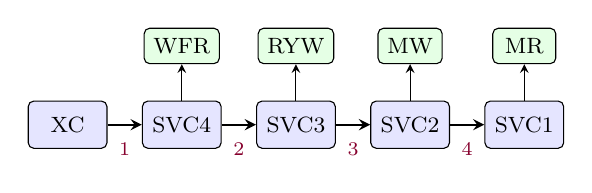
\begin{tikzpicture}[
    font=\footnotesize,
    node distance=1.45cm,
    service/.style={draw, rounded corners=2pt, fill=blue!10, minimum width=1.0cm, minimum height=0.6cm, align=center},
    semantic/.style={draw, rounded corners=2pt, fill=green!10, minimum width=0.8cm, minimum height=0.45cm, align=center},
    arrow/.style={->, >=stealth, thick},
    semantic_arrow/.style={->, >=stealth, thin},
    app/.style={font=\scriptsize, text=purple!70!black}
  ]

  % stacked services
  \node[service] (xc)   at (0,0) {XC};
  \node[service] (svc4) [right of=xc] {SVC4};
  \node[service] (svc3) [right of=svc4] {SVC3};
  \node[service] (svc2) [right of=svc3] {SVC2};
  \node[service] (svc1) [right of=svc2] {SVC1};

  % arrows from services to semantics
  \node[semantic] (wfr) [above of=svc4, node distance=1.0cm] {WFR};
  \node[semantic] (ryw) [above of=svc3, node distance=1.0cm] {RYW};
  \node[semantic] (mw)  [above of=svc2, node distance=1.0cm] {MW};
  \node[semantic] (mr)  [above of=svc1, node distance=1.0cm] {MR};

  % edges
  \draw[semantic_arrow] (svc4) -- (wfr);
  \draw[semantic_arrow] (svc3) -- (ryw);
  \draw[semantic_arrow] (svc2) -- (mw);
  \draw[semantic_arrow] (svc1) -- (mr);

  % edge constraints
  \draw[arrow] (xc) -- (svc4)   node[midway, below=0.1cm, app] {1};
  \draw[arrow] (svc4) -- (svc3) node[midway, below=0.1cm, app] {2};
  \draw[arrow] (svc3) -- (svc2) node[midway, below=0.1cm, app] {3};
  \draw[arrow] (svc2) -- (svc1) node[midway, below=0.1cm, app] {4};

\end{tikzpicture}
\caption{Cross-service causal composition chain. Edge labels mark the application-level semantic ``glue'' added per hop, e.g., XC$\to$SVC4 supplies the missing guarantees (MR+MW+RYW) to reach causal consistency, and the downstream edges do likewise for their missing session guarantees. Per-level storage nodes provide guarantees for each service layer.}
\label{fig:cross-service-causal}
\end{wrapfigure}

Cross causal (XC) storage~\cite{boltoncc} combines
multiple distributed storage services, each
offering only a basic consistency guarantee, to provide causal consistency
as a whole (\cref{fig:cross-service-causal}). 
As XC storage itself is a system, its constraints are very different from application-level constraints in previous case studies;
XC storage showcases the capability of \sysname{} beyond modeling application logics.

Users accessing data through the XC node get causal consistency,
but individual storage DB maintains weaker semantics than causal.
SVC4 node's storage backend only provides WFR. To achieve causal
consistency, application places a shim layer to strengthen the semantics
in the design and this is imposed on the edge between SVC4 and XC.
While the SVC4-XC combination can achieve causal consistency, SVC4's
downstream service SVC3's storage backend only provides RYW. To achieve
cross-system causal consistency, the augmentation continues down the chain.

%This example demonstrates modeling a system where multiple services, each
%offering only a basic consistency guarantee, are chained together.

The goal here is to verify whether their composition, mediated by specific
inter-service
constraints, symbolic isolation, and the role of explicit ``glue'' constraints.

\para{Architecture.} The architecture forms a chain $\text{XC} \rightarrow
\text{SVC4} \rightarrow \text{SVC3} \rightarrow \text{SVC2}
\rightarrow \text{SVC1}$.
Each service $\text{SVC}n$ ($n=1..4$) is designed to provide only
\textit{one} of the
four session guarantees via its \texttt{provs} attribute:
$\text{SVC}1$ provides MR, $\text{SVC}2$ provides
MW, $\text{SVC}3$ provides RYW, and $\text{SVC}4$ provides WFR.

\para{Constraints Encoding and Compatibility Verification.}
%\textbf{Symbolic Isolation:}
To prevent logical interference, the guarantee provided by
each service and the constraints added on the edges are instantiated
using unique
symbols specific to that service or edge.
This ensures, for example, that the MR constraints of
$\text{SVC}1$ only apply to operations symbolically designated as belonging to
$\text{SVC}1$.

%\textit{Composition via Edge Constraints:}
The composition logic resides in the ``glue''
constraints defined on the \texttt{cons} attribute of the edges connecting the
services. Since each service node only provides one session
guarantee, the edge $\text{SVC}n \rightarrow \text{SVC}(n+1)$ must
provide constraints representing the other three session guarantees needed to
potentially satisfy causal consistency up to that point.

The core idea of this example is to build a stronger guarantee by composing
weaker guarantees provided by individual services ($\text{SVC}1
\ldots 4$), using
the edges to supply the missing pieces which reflects the application design
as shown in \cref{fig:cross-service-causal}.

%\begin{itemize}
%\item $\text{SVC}1$ provides only MR via its storage backend.
%\item To achieve Causal Consistency when accessing data through $\text{SVC}2$,
%  the edge between $\text{SVC}1$ and $\text{SVC}2$ must
%  provide the missing session guarantees: MW, RYW, and WFR through
%  application-level business logic.
%\item Similarly, $\text{SVC}2$ provides only MW via its storage
%  backend. To maintain Causal Consistency
%  when accessing data through $\text{SVC}3$, the edge between
%  $\text{SVC}2$ and $\text{SVC}3$ must
%  provide MR, RYW, and WFR.
%\item This pattern continues: $\text{SVC}3$ provides RYW, so the edge
%  to $\text{SVC}4$ must provide MR, MW, and WFR.
%\item Finally, $\text{SVC}4$ provides WFR, so the edge to $\text{XC}$
%  must provide MR, MW, and RYW.
%\item The $\text{XC}$ node serves as the extraction point where users
%  can access data with full causal consistency guarantees.
%\end{itemize}

%\textit{Symbol Equivalence:}
For this composition to be meaningful in the SMT-solver-based
\sysname{}, we must
conceptually link operations across services that refer to the same logical
action or data. For instance, if write $w_1$ in $\text{SVC}1$ and
write $w_2$ in $\text{SVC}2$ both
represent updates to the same user profile, ``glue'' constraints
equating relevant
aspects (like $w_1.\text{obj} = w_2.\text{obj}$ or $w_1.\text{ival} =
w_2.\text{ival}$ despite their different symbolic names) is necessary.
While the current test code
simplifies this by focusing on composing the consistency axioms, a more rigorous
model would include these explicit symbol equivalence constraints on the edges
(we are asserting symbols of $w_1$ are identical to those of $w_2$ for
simplicity).

%\textit{Aggregation:} The \texttt{composable(g, svc1)} call attempts
%to find a satisfying
%assignment for the entire chain, respecting the \texttt{provs} of
%each node and the \texttt{cons} of
%each edge. If it returns \texttt{True}, it confirms that the
%individual guarantees can
%be composed under the specified edge constraints. Subsequently,
%\texttt{extract(svc1, svc1, (ok, res))} can

After a single logical formula representing the net end-to-end guarantee
achieved by the SVC chain is synthesized starting from $\text{SVC}1$
to XC, the formula is then compared against a formal definition of CC
to verify compatibility, which succeeds. While
the original XC implementation~\cite{boltoncc} ties together only EC
storage services, this example further explores more diverse storage
services and demonstrates the flexibility of \sysname{}.
With the successful compositional check, the multi-node XC chain can be
collapsed into a single entity (similar to how Login + User DB could be summarized)
by applying \texttt{extract} to the full XC graph.
This yields one aggregated \texttt{provs}/\texttt{needs} tuple representing
the composed cross storage system causal consistency guarantee for any future downstream use.

%\subsubsection{Interaction Flows}
%
%The media streaming service supports several interaction patterns,
%each with specific consistency requirements:
%
%\textbf{User Registration and Authentication}: Before accessing any
%content, users must register and authenticate through the login
%service. This process involves:
%
%\begin{enumerate}
%\item The client sends a registration request (abstracted as a
%  write operation) to the login service.
%\item The login service writes the new user credentials to the User Database.
%\item For subsequent logins, the client sends a login request
%  (abstracted as a read operation) to the login service.
%\item The login service reads from the User Database to verify credentials.
%\end{enumerate}
%
%The MW and WFR guarantees of the User Database ensure that once user
%credentials are updated, all subsequent authentication attempts will
%see the updated information, preventing authentication anomalies
%where users might be unable to log in with newly created or changed
% credentials.
%
%\textbf{Browsing and Playback}: Once authenticated, users can browse
%and watch available content:
%
%\begin{enumerate}
%\item The client sends a request to browse content, which queries
%  the Metadata Database.
%\item When a user selects content to watch, the client sends a
%  request to the Video Service.
%\item The Video Service verifies the content's existence and
%  availability by reading from the Metadata Database.
%\item If the content is available, the Video Service streams the
%  content from the Video Database to the client.
%\end{enumerate}
%
%The MR guarantee of the Video Service ensures that once a piece of
%content is determined to be available, subsequent read operations
%will maintain this view, preventing inconsistencies during playback.
%The WFR guarantee of the Video Database ensures that if the service
%reads a specific version of content, subsequent writes will not
%revert to an earlier version.
%
%\textbf{Rentals}: For premium content, users must first rent the content:
%
%\begin{enumerate}
%\item The client sends a rental request to the Rent Service.
%\item The Rent Service checks content availability by reading from
%  the Metadata Database.
%\item If available, the Rent Service records the transaction in the
%  Rent Database.
%\item The client can then access the rented content through the Video Service.
%\end{enumerate}
%
%The MR guarantee of the Rent Service ensures consistent inventory
%checks, preventing scenarios where content appears to be available
%and then becomes unavailable during the rental process.
%
%\textbf{Reviews}: Users can read and write reviews for content they've watched:
%
%\begin{enumerate}
%\item To read reviews, the client sends a request to the Review
%  Service, which retrieves reviews from the Review Database.
%\item To write a review, the client sends the review content to the
%  Review Service.
%\item The Review Service verifies that the content exists by
%  reading from the Metadata Database.
%\item If verified, the Review Service writes the review to the
%  Review Database.
%\end{enumerate}
%
%The RYW guarantee of both the Review Service and Review Database
%ensures that users immediately see their own reviews after
%submission, providing a responsive user experience while allowing for
%eventual consistency for other users' views.
%
%\textbf{Admin Operations}: Administrators manage content through
%separate workflows:
%
%\begin{enumerate}
%\item Administrators authenticate through the Login Service (with
%  pre-granted access).
%\item To add new content, administrators:
%  \begin{itemize}
%    \item Upload video content to the Video Database through the
%      Video Service.
%    \item Add corresponding metadata to the Metadata Database.
%  \end{itemize}
%\item To modify user accounts, administrators interact with the
%  Login Service, which updates the User Database.
%\end{enumerate}
%
%The combination of RYW and MR guarantees in the Metadata Database
%ensures that administrative updates are immediately visible to the
%administrators themselves while allowing for controlled propagation
%to user-facing services.
%

\section{Evaluation} \label{sec:eval}

We discuss our experience in using \sysname{} and
its performance in checking compatibilities.

\newcommand{\tableT}{\textcolor{blue}{T}}
\newcommand{\tableF}{\textcolor{red}{F}}
\newcommand{\tableNA}{-}
%\begin{wraptable}[13]{R}{3.4in}
\begin{wraptable}{R}{3.4in}
  \centering
  \small
  \caption{Pairwise check performance. Semantics in the first column
    are checked if they satisfy semantics in other columns. Each cell
    shows the execution time for completing the check in milliseconds. The
  blue text indicates the check result is true and red means false. }
  \label{tab:pairwise-time}
  \begin{tabular}{|l|c|c|c|c|c|c|c|c|}
    \hline
    {} &
    EC &
    MR &
    MW &
    RYW &
    WFR &
    PRAM &
    CC &
    LIN \\
    \hline
    EC   & \tableNA & \textcolor{red}{24} & \textcolor{red}{22} &
    \textcolor{red}{26} & \textcolor{red}{25} & \textcolor{red}{24} &
    \textcolor{red}{35} & \textcolor{red}{32} \\
    MR   & \textcolor{blue}{23} & \tableNA & \textcolor{red}{12} &
    \textcolor{red}{16} & \textcolor{red}{75} & \textcolor{red}{16} &
    \textcolor{red}{26} & \textcolor{red}{217} \\
    MW   & \textcolor{blue}{27} & \textcolor{red}{16} & \tableNA &
    \textcolor{red}{18} & \textcolor{red}{16} & \textcolor{red}{16} &
    \textcolor{red}{23} & \textcolor{red}{22} \\
    RYW  & \textcolor{blue}{193} & \textcolor{red}{106} &
    \textcolor{red}{45} & \tableNA & \textcolor{red}{59} &
    \textcolor{red}{20} & \textcolor{red}{29} & \textcolor{red}{26} \\
    WFR  & \textcolor{blue}{24} & \textcolor{red}{125} &
    \textcolor{red}{12} & \textcolor{red}{17} & \tableNA &
    \textcolor{red}{18} & \textcolor{red}{44} & \textcolor{red}{54} \\
    PRAM & \textcolor{blue}{24} & \textcolor{blue}{14} &
    \textcolor{blue}{10} & \textcolor{blue}{14} &
    \textcolor{red}{178} & \tableNA & \textcolor{red}{27} &
    \textcolor{red}{28} \\
    CC   & \textcolor{blue}{33} & \textcolor{blue}{20} &
    \textcolor{blue}{16} & \textcolor{blue}{19} &
    \textcolor{blue}{19} & \textcolor{blue}{20} & \tableNA &
    \textcolor{red}{282} \\
    LIN  & \textcolor{blue}{26} & \textcolor{blue}{21} &
    \textcolor{blue}{17} & \textcolor{blue}{22} &
    \textcolor{blue}{22} & \textcolor{blue}{22} &
    \textcolor{blue}{44} & \tableNA \\
    \hline
  \end{tabular}
\end{wraptable}
%\vspace{-0.3in}

\para{Experience.}
We implemented \sysname{} in Python on Z3 version 4.15.1. It took
approximately 3.7K lines of code to implement \sysname{}. 
%
%% \textbf{Usability}
%% During review, on several instances we were asked on the usability of \sysname.
%% We summarized them in these 3 main categories: how can the framework be used,
%% the expected user input and effort,
%% and the scalability of our methodology in large-scale applications.
% 1
To use \sysname{}, users supply \sysgraph whose nodes and/or edges carry
built-in or custom \sysmods that extend the base model and relation interfaces.
When multiple \sysmods are attached, \sysname checks the given
input or exhaustively explores valid combinations.

%The \texttt{check} function optionally emits proof goals via the \texttt{witness} argument (see \texttt{tests/test\_witness.py} in the accompanying artifact), which can be discharged to external SMT solvers.

% 2
Regarding effort and the learning curve, once semantic requirements are understood, encoding an \sysgraph is straightforward.
Our case studies only require 183, 80, and 252 lines of code for encoding the movie streaming service, online shopping mall, and XC storage, respectively, thanks to existing facilities such as the \sysmods{} in the \sysname{} framework. 
These relatively small efforts for constraint encoding and automated checks validate our framework's goal of enabling agile compatibility checks compared to typical end-to-end formal verification which could have huge proof-to-code/specification ratio~\cite{certikos-osdi16, klein2009sel4, wormspace, ironfleet, disel} which could follow with confidence after our \sysname{} check passes. 
%Our effort constraints remain stable unless interfaces or consistency requirements change.

% 3
The scalability of our tool is mainly expressed via modular composition,
\sysgraph nodes and edges compose modularly: large systems can be decomposed into sub-\sysgraphs,
verified independently, and re-aggregated into a monolithic node that preserves the verified properties of its components.
This pattern (\eg Case Study 2 in Section \ref{sec:cs}) also enables parallel SMT solving on sub-components and 
reuse of solved results for large service meshes.
%(see \texttt{tests/test\_aggregate.py} and Case Study 2 in Section \ref{sec:cs}) also enables parallel SMT solving on sub-components and reuse of solved results for large service meshes.

% end
In general, our framework offers early compatibility detection,
architecture validation before implementation, and pre-verification screening to de-risk downstream formal proofs.
It targets teams building correctness-critical distributed systems who want a high-level, low-maintenance checker rather than line-by-line deductive proof development (\eg using tools like Verus\cite{verus}, Dafny\cite{dafny}, Rocq\cite{coq}, and Lean\cite{lean}).


\para{Performance.}
SMT solvers often take an extended period to complete their tasks.
Thus, we measure the
duration of the compatibility check in \sysname{}.
All experiments were conducted on an Intel i7-1360P processor with
64\,GB RAM running NixOS 25.11 (Linux 6.12.30).

% 10 seconds
% timeout limit. However, during our evaluation, we discovered a
% termination bug in Z3 4.15.1
% where the solver would not respect timeout parameters, continuing to
% run well beyond the specified limit (e.g., still running after 2
% minutes despite a 10-second timeout). To address this, we implemented
% a watchdog mechanism using strace to monitors write systemcalls to
% stdout, sending SIGINT if the 10-second timeout is exceeded,
% following the philosophy established in recent
% verification work Verus that ``it's better to improve solver
% performance than rely on a slow proof'' \cite{verus}.
% https://github.com/verus-lang/verus/blob/0b6f3cbb8fceff6681b4988c3cac37a8b801f8e6/source/docs/guide/src/smt_failures.md

\textbf{Pairwise Compatibility Check.}
%
First, we evaluated the compatibility between pairs of base
consistency semantics,
EC, MR, RYW, MW, WFR, PRAM, CC, and LIN, in \sysname{}.
Table \ref{tab:pairwise-time} shows the execution times for these
pairwise compatibility checks and the results of the check encoded in
colors (blue: compatible, red: non-compatible). On average, it took
only 31 ms per check and the results of the checks are correct with
respect to the theory.


%\begin{wraptable}[9]{R}{3.37in}
\begin{wraptable}{R}{3.37in}
	\center
	\small
	\caption{Search time for compatible DMs. Columns show number of searched DM combinations, time to search all combinations (all), time to find the minimum score combination (min score), and average time to check one combination (single).  ($^*$ predicted time)}
	\label{tbl:searchtime}
	\begin{tabular}{ |l|r|r|r|r| }
		\hline
		Application & \# of combs. & All & Min score & Single \\
		\hline
		Movie    & $17^5=1.4\textrm{M}$ & 64.82 hr$^*$ & 20.43 sec  & 164.4 ms\\
		Shopping & $17^3=4.9\textrm{K}$ &251.77 sec   & 1.65 sec   & 51.25 ms \\
		XC store & $17^4=83.5\textrm{K}$ &3.98 hr      & 261.09 sec & 171.7 ms\\
		\hline
	\end{tabular}
%	\end{table}
\end{wraptable}
\textbf{Compatible \sysmod{} Search.} Next, we evaluate \sysname{} using
three case studies in \cref{sec:cs}.
This evaluation focuses on two key metrics: the framework's ability to
find valid compositions with the weakest semantics (i.e., the minimum score combination in \cref{subsec:search}) and its
performance characteristics under different system complexities.
%
For each case study, we gave blank \sysmods{} to each application
so that \sysname{} searches and outputs compatible \sysmod{} combinations.
\sysname{} uses the search strategy in \cref{subsec:search}. The results are summarized in \cref{tbl:searchtime}.
%we enumerated all possible combinations of
%consistency models for nodes with non-null provs fields, while
%keeping nodes with predefined needs fields unchanged. We assigned
%scores to individual consistency models and their combinations based
%on their strength as shown in Figure \ref{fig:semantics-tree}.

Movie streaming service requires finding \sysmods{} corresponding to
five DB nodes that satisfy application node and edge constraints.
Given that \sysname{} contains 17 \sysmods{} as illustrated in
\cref{fig:semantics-tree} the full search space contains
$17^5$ combinations. On average, checking each combination
takes 164.4 ms and can find a compatible combination with the lowest
score in 20.43 seconds with a timeout of 10 seconds for each check.
Checking the entire search space is feasible but is expected to take
64.82 hours (we have completed 800,507 checks or 56.38\% of the search space
in 36.55 hours).

The online shopping mall example is simpler than the movie streaming service
and involves only three DB nodes to search.
We evaluated all $17^3$ possible combinations of consistency semantics across
these nodes. The evaluation completed in 251.77 seconds with an average
duration of 51.25 ms per combination with 0 timeouts. The minimum score combination 
was found in 1.65 seconds. 

Finally, four DB node combinations (i.e., $17^4$ cases) are searched for
the cross causal storage. The total search completes in 3.98 hours
with an average duration of 171.7 ms per combination.
Our tool successfully identified the combination in our original design (also the
minimum score combination) in about 261.09 seconds. The timeout rate is only about 0.15\% of cases.

Overall, depending on the complexity of the constraints the
compatibility check times
vary, but individual checks are done in less than 200\,ms on average. Even though
searching through compatible answers in the entire search space could
take extended
time, finding the optimal, minimum-score configuration for each case
study takes only less than 5 minutes.



\section{Related Work}

Our work sits at the intersection of distributed systems, formal
verification, and automated reasoning.
We organize the related work into consistency verification
frameworks, SMT-based approaches
for distributed systems, and compositional analysis tools.

Several frameworks have been developed to verify consistency
properties in distributed systems.
Quelea \cite{sivaramakrishnan2015declarative} provides a declarative
programming model where developers
specify consistency requirements as contracts using a shallow
extension of Haskell and discharge proof obligations to SMT solvers.
The system then automatically selects appropriate consistency levels.
However, Quelea focuses on single-system consistency rather than
cross-service composition and relies on conservative
approximations of happens-before relationships due to limitations in
expressing transitive closures in first-order logic.

Jepsen \cite{kingsbury2025jepsen} takes a different approach by
performing black-box testing of
distributed systems to detect consistency violations through
controlled fault injection. While
effective at finding bugs in real systems, Jepsen cannot provide
formal guarantees about system
compositions or verify that specific consistency requirements are met by design.

The use of SMT solvers for distributed systems verification has
gained traction in recent years.
Kuper et al. \cite{kuper2019toward} argue for domain-specific solvers
embedded in solver-aided
languages like LiquidHaskell and Rosette to build
consistent-by-construction applications.
They identify key challenges including CRDT verification, message
reordering analysis, and transitive
closure reasoning. While they advocate for specialized solvers, our
work demonstrates that careful encoding
strategies can make general-purpose SMT solvers effective for
consistency verification.

Fan et al. \cite{fan2023satisfiability} develop an ordering
consistency theory for verifying
multi-threaded programs under memory models like sequential
consistency and TSO. Their approach
uses incremental consistency checking and specialized theory
propagation to efficiently handle
ordering constraints. Although focused on memory models rather than
distributed consistency,
their formalization of ordering relations ($\prec_{rf}$,
$\prec_{fr}$, $\prec_{ws}$) provides insights
for our visibility-based encoding of session guarantees.
More recently, Kater~\cite{kater} expresses weak memory consistency models in a
fragment of Kleene algebra with tests, automatically answers metatheoretic
questions about them, and generates consistency checkers. While Kater targets hardware and language memory models rather
than the service-composition setting of \sysname{}, its algebraic treatment of
ordering relations is closely related to our relational encoding of visibility
and session guarantees.

MixT~\cite{mixt} is a domain specific language to simplify
programming mixed-consistency transactions over multiple
distributed systems. It uses information flow theory to
generate transactions consisting of sub-transactions
that safely execute across multiple systems with different
semantics. While MixT is a specialized tool to generate
safe and efficient transactions for given consistency semantics
of distributed systems, \sysname{} allows developers to check
correctness of their operations over chosen combination of
distributed systems or search for compatible consistency
semantic combinations.

\sysname{} differs from existing approaches in several ways:
unlike single-system verification frameworks,
we focus specifically on the composition problem where services with
different consistency models work together; unlike testing-based
approaches, we provide formal compatibility checks over different semantics;
unlike theorem-proving approaches, we use automated reasoning to make
the verification process more accessible to practitioners.

Our encoding strategy addresses limitations identified in prior work
by avoiding explicit reasoning about global event orderings and
instead treating consistency as logical constraints over abstract
executions. This approach makes the verification tractable
while remaining expressive enough to handle realistic service
compositions. Our framework's ability to synthesize end-to-end
guarantees from component specifications provides developers and
system architects with actionable insights about their systems'
consistency behavior.

% rework
% [high prio] mixt paper
% [low prio] add smt for coverage checking paper

% \section{Toward Domain-Specific Solvers for Distributed Consistency}
%
% \subsection{Summary}
%
% In Kuper et al. \cite{kuper2019toward}, the authors argued
% embedding automated theorem
% solvers into a language like
% LiquidHaskell \cite{vazou2014liquidhaskell} and Rosette
% \cite{torlak2014a}, and use these solver-aided languages implement
% distributed systems
% can result in consistent-by-construction applications. However, transitive
% relations, partial orderings, and external API invocations are difficult
% properties to reason in these solver-aided languages due to non-trivial
% encodings and efficiency concerns. The authors advocates for developing
% domain-specific SMT solvers that are specialized for reasoning
% about distributed
% consistency properties, and programmers should not need to fully understand
% satisfiability modulo theories in order to implement theory solvers for their
% domain of interest with the help of these domain-specific solver frameworks.
%
% \subsection{Methodology}
%
% The paper presents a vision rather than a specific implementation, drawing on
% experiences with existing systems to motivate the need for domain-specific
% solvers. The methodology focuses on identifying key challenges and outlining a
% research agenda rather than providing concrete solutions.
%
% The authors listed three key features a "consistency-aware" solver
% should have:
%
% \begin{itemize}
%   \item CRDT verifications: current verification of CRDT properties
%     in Liquid Haskell
%     requires non-trivial encodings and takes up to 40 seconds for
%     basic ordering
%     laws.
%
%   \item Message reorderings: for lineage-driven fault injection
%     (LDFI), the ability to
%     efficiently reason about message commutativity could enable
%     exploration of bugs
%     triggered by message races while avoiding state explosion.
%     Personally, this does
%     not seem to be a target area for our work.
%
%   \item Transitive closures: in
%     Quelea \cite{sivaramakrishnan2015declarative}, the inability
%     to precisely express transitive closure in first-order logic forces overly
%     conservative approximations of happens-before relationships.
%     While this is a
%     very valid, and on-point concern, however, transitive closures
%     are encodable in
%     solver frameworks with quantifiers elimination tactics and
%     recursive definitions
%     (which are standards in
%     SMT-LIB\footnote{https://smt-lib.org/papers/smt-lib-reference-v2.6-r2017-07-18.pdf}).
% \end{itemize}
%
% \subsection{Relavance}
%
% On a first glance, the paper seem to reject our thesis where we did used
% general-purpose SMT solvers like Z3 \cite{demoura2008z3} to reason
% about distributed
% consistency properties. Throughout the development of our framework, we have
% encountered the same issues as the authors mentioned, where the encoding of
% transitive relations, partial orderings, and non-deterministic operations are
% non-trivial and inefficient.
%
% However, rather than rejecting general-purpose solvers entirely, our work
% demonstrates that careful encoding strategies and abstraction choices can help
% mitigate some of these limitations. We take inspiration from the
% paper's vision
% of domain-specific solvers while working within the constraints of existing
% tools.
%
% Instead of trying to deduce a global ordering of events from a set of axioms
% (not decidable in the first place), we avoid explicit reasoning about state
% machine transitions (i.e. explicit version vectors or Lamport clocks), our
% framework treats consistency guarantees as logical constraints over abstract
% executions. The checking call to solvers reduces verification to constraint
% satisfaction problems (negation of implication) that are decidable in
% first-order logic. However, we acknowledge that domain-specific solvers as
% proposed could potentially make our approach even more efficient.
%
% \section{Satisfiability Modulo Ordering Consistency Theory for SC,
% TSO, and PSO Memory Models}
%
% \subsection{Summary}
%
% Fan et al. \cite{fan2023satisfiability} propose a ordering
% consistency theory for
% verifying multi-threaded programs under sequential consistency
% (SC), TSO and PSO
% (total/partial store order) memory models. While partial orders can concisely
% represent thread interleavings, existing approaches using integer difference
% logic to encode ordering constraints are inefficient as they: compute exact
% clock values when only relative ordering matters, and eagerly encode all
% possible from-read orders (read-from and from-read are extramely
%   similar to our
% visible/visibility definition) regardless of whether they are needed. The
% authors develop a theory solver that performs incremental
% consistency checking,
% generates minimal conflict clauses, and includes specialized theory
% propagation.
%
% \subsection{Methodology}
%
% The paper formalizes their ordering consistency theory
% $\mathcal{T}_{ord}$ with
% signature where (Section 4.1):
%
% $$
% \Sigma_{ord} = \{ e_1, e_2, ..., \prec_{ppo}, \prec_{ws},
% \prec_{rf}, \prec_{fr}, \approx \}
% $$
%
% \begin{itemize}
%   \item $e_i$ are memory access events in $EE$
%   \item $\prec_{ppo}$ represents preserved program order (binary predicate)
%   \item $\prec_{ws}$ represents write serialization (binary predicate, total
%     order of writes to same address)
%   \item $\prec_{rf}$ represents read-from relation (binary predicate,
%     linking writes to reads)
%   \item $\prec_{fr}$ represents from-read relation (binary predicate,
%     derived from $\prec_{ws}$ and $\prec_{rf}$)
%   \item $\approx$ represents atomicity equivalence relation
% \end{itemize}
%
% Where the 4 axioms of $\mathcal{T}_{ord}$ are:
%
% \begin{itemize}
%   \item partial order where $\prec_{ws}$ only relates write events,
%     $\prec_{rf}$ link
%     write events to read events, and $\prec_{fr}$ link read events to
%     write events
%   \item equivalence relation (trivial reflexivity)
%   \item from-read derivation where it's similar to our monotonic
%     read definition
%     (visibility included)
%   \item consistency where $\prec_{ws} \cup \prec_{rf} \cup \prec_{fr}$ is
%     consistent with $\prec_{ppo}$ and $\approx$
% \end{itemize}
%
% The solver maintains an event graph (think of this as abstract
% executions) where
% nodes are events and edges represent ordering relations. Rather than eagerly
% encoding all possible from-read orders, it derives them on-demand
% during solving
% when relevant variables are assigned. Consistency checking reduces to cycle
% detection in this graph.
%
% The solver performs incremental cycle detection by maintaining a
% pseudo-topological order of events and updating it efficiently when edges are
% added. When inconsistency is detected, it generates minimal
% conflict clauses by
% finding critical cycles with the smallest number of induced edges. This
% formalization aligns closely with our visibility/visible definitions (and
% session semantic definitions), but they treat read-from and from-read as
% separate relations rather than doing explicit case analysis and combining them
% into a single visibility relation.
%
% \subsection{Relavance}
%
% The paper's formalization approach provides important insights for our work.
% Their rigorous axiomatization of ordering relations provides a
% template for how
% we could formalize our consistency models more precisely (instead of using
% proses like how we have).
%
% While we focused on higher-level consistency specifications rather than
% low-level memory model semantics, and considering we combined read-from and
% from-read into a single visibility relation with case analysis rather than
% treating them separately, this paper demonstrates the benefits of having a
% precise formal theory with clear axioms and efficient decision
% procedures. Even
% though the domain is different, many of their theoretical techniques could
% potentially be adapted to make our framework more rigorous and efficient.
%
% Couple points to note: we should take their pseudocode example and layout our
% checking logic. They also made Fig. 3 to demonstrate the differences of event
% graphs constructed from different relations, we should also consider this to
% show the case analysis for visibility definition For application
% level checking,
% Fig. 5 and Fig. 6 should be taken into consideration, and we should implement
% SMT-LIB exporter to make our tool checker agnostic. The paper also have
% experiments on evaluations, we should also consider this.

\section{Conclusion}

In this paper, we presented \sysname{}, the first automated framework
for checking semantic compatibility between applications and
compositions of distributed systems with different consistency
guarantees.  Our key contributions include formal definitions of
distributed consistency semantics including the first rigorous formal
definition of visibility, the \sysgraph{} modeling approach for
systematic encoding of microservice-like applications, and an
SMT-based compatibility checking framework that can check
compatibility between given distributed semantics and applications
and search for compatible combinations of distributed semantics for
the application. Through case studies on three distributed
applications, we demonstrated that \sysname{} can model and verify
complex service compositions with little encoding effort while
providing formal guarantees about system correctness.  As distributed
system architectures grow increasingly complex, \sysname{} provides
developers with essential tools for quickly checking the integrity of
the distributed application designs, enabling more agile system design
where components can be modified or replaced with confidence.


\section*{Data Availability}
The artifact accompanying this paper is available on Zenodo~\cite{ourartifact}.

\begin{acks}
We thank the anonymous reviewers for their insightful reviews. This work is partially supported by \grantsponsor{NSF}{NSF}{https://www.nsf.gov} award \#\grantnum{NSF}{2442888}.
\end{acks}

\bibliographystyle{ACM-Reference-Format}
\bibliography{references, refs2}


\end{document}
